\documentclass[11pt,a4paper]{scrreprt}

% Codierung
\usepackage{selinput}
\SelectInputMappings{
  adieresis={ä},
  germandbls={ß},
}
\usepackage[ngerman]{babel}
\usepackage[T1]{fontenc}
\usepackage{lmodern}

% Kopf-/Fusszeilen
\usepackage{scrlayer-scrpage}
\usepackage{lastpage}
\setkomafont{pageheadfoot}{\small\sffamily}
\pagestyle{scrheadings}
\lohead*{}
\cohead*{}
\rohead*{}
\lofoot*{ITPMF}
\cofoot*{}
\rofoot*{Seite \thepage \hspace{1pt} von \pageref{LastPage}}

\usepackage{lipsum}

% Bilder
\usepackage{graphicx}

% Hyperlinks
\usepackage[hidelinks]{hyperref}

\begin{document}
\titlehead{Hochschule Luzern \\ 
	Technik \& Architektur}
\subject{Zusammenfassung}
\title{IT-Projektmanagement \& Führung}
\subtitle{}
\author{Fabian Wüthrich \\ 
	Simon Erni \\ 
	Alex Suter}
\date{\today}

\maketitle

\tableofcontents

\chapter{Einführung}

Nur BlaBla nichts was an der Prüfung kommt...

\chapter{Wahrnehmung \& Kommunikation}

Jede Interaktion mit der Welt setzt voraus, dass wir die Welt überhaupt wahrnehmen. Das Experiment \textit{Blinder Fleck} zeigt, dass wir die Welt offenbar falsch wahrnehmen.

Unsere Sensoren nehmen Reize wahr und gehen mittels Neuronen übers Rückenmark ans Gehirn. Die Körpergrenze ist das Interface. Siehe dazu auch das Bild in Kapitel Selbstführung \ref{fig:neurale-informationverarbeitung}. Alle Informationen gelangen ins UB, nur ein Teil davon ins Bewusstsein. Geruchs- und Geschmacksinfos können wir nicht filtern. Aktuelle Infos werden mit vorhanden Infos (Gedächtnis) gemischt.

\section{Vom Sehen zum Bild}
\begin{enumerate}
	\item Elementarformen identifizieren. Wir nehmen zuerst folgendes wahr: Kante, Form, Farbe, Flächen, Bewegungen, Gesichter ...
	\item Anschliessend verdichten wir zu Gebilden, wie: Gebäude, Orte, Geräte, Objekte ...
	\item Mustererkennung. Wir assoziieren das Objekt mit Erinnerungen.
\end{enumerate}

\paragraph{Zeitliche Koordination:}
Übertragung der sensorischen Impulse dauert unterschiedlich lange (Fuss-Gehirn, Auge-Gehirn). Für Verarbeitung der Information benötigt das Gehirn unterschiedlich viel Prozessorzeit (Formen/Farben/Texte etc.). Um alles zu einem Gesamtbild zusammenzusetzen, muss es auf den langsamsten Prozess warten. Alle Reize innert 100ms ... 120ms betrachtet das Gehirn als zusammengehörend. 

\paragraph{Wahrnehmung geschieht unbewusst:}
Der grösste Teil der Wahrnehmung geschieht unbewusst und kann vom Bewusstsein nicht beeinflusst werden. Was dem Bewusstsein als Wahrnehmung präsentiert wird, ist eine vom UB aufgebaute, scheinbare plausible Story. Auf die Story haben Erwartungen, Hoffnungen, Erinnerungen genauso starken Einfluss wie die effektiven Umweltreize.

Merksatz: ''Wir glauben, was wir sehen, weil wir sehen, was wir glauben''

\paragraph{Evolution:} [MEP] Die Wahrnehmung hat sich über die gesamte Zeitspanne der Evolution entwickelt. Evolution ist in jedem von uns drin. Jeder Mensch durchläuft abgekürzt die gesamte menschliche Evolution. Auch das Gehirn hat sich entwickelt, die einzelnen Gehirnteile sind übereinander gewachsen:

\begin{description}
	\item[Stammhirn:] aka Krokodil. Schon bei Reptilien \& Vögeln und steuert automatische Reflexe und Körperfunktionen.
	\item[Limbisches System:] aka Pferd aka Zwischenhirn. Frühe Säugetiere und ist für Gefühle und unbewusste Reaktionen verantwortlich.
	\item[Neocortex:] aka Delphin aka Grosshirn. Höhere Säugetiere, Primaten dient für rationales Denken, Vernunft und bewusste Entscheidungen.
	\item[Präfrontaler Cortex:] aka Guru aka Stirnhirn. Menschen, ab ~16j und ist für Mathematik, Kreativität, Meditation etc. da.
\end{description}

Unser Gedächtnis beginnt nicht leer. In jedem von uns sind die nützlichen Erfahrungen unserer Vorfahren bereits verankert. Die jüngsten Erfahrungen (ca. vor 8000 Jahren), Ackerbau und Viehzucht sind bereits zu einem klein Teil körperlich verankert. Das individuelle Gedächtnis ergänzt lediglich eine enorme Menge bereits vorhandener Erinnerungen.

\paragraph{No database:}
Achtung - Das Gedächtnis ist keine Datenbank. Wir speichern nur Bruchstücke. Bei jedem Lese Zugriff auf eine Erinnerungen, nehmen wir diese, und speichern sie meist modifiziert wieder ab. Die Erinnerungen ist ein unzuverlässiges Konstrukt. Tipp von Ernst: Dann modifiziere Sie doch einfach in die bessere Richtung.

\section{Fazit}
Was sich uns als Realität darstellt ist ein vom Unterbewusstsein aus neu eingehenden Informationen, Erinnerungen, Erfindungen und Streichungen
zusammengemischtes, ~100 mS altes Konstrukt.
\begin{itemize}
	\item Wir sehen die Realität, die wir sehen wollen
	\item Was wir sehen wollen, hängt ab von unseren früheren Erlebnissen, aktuellen Erwarutngen und unseren tiefliegenden Glaubensätzen.
	\item Die Konstruktion der Realität erfolgt unbewusst.
\end{itemize}

[MEP] In der Abbildung \ref{fig:wahrnehmung-ablauf} sehen wir den Ablauf der Wahrnehmung.

\begin{figure}[h!]
\centering
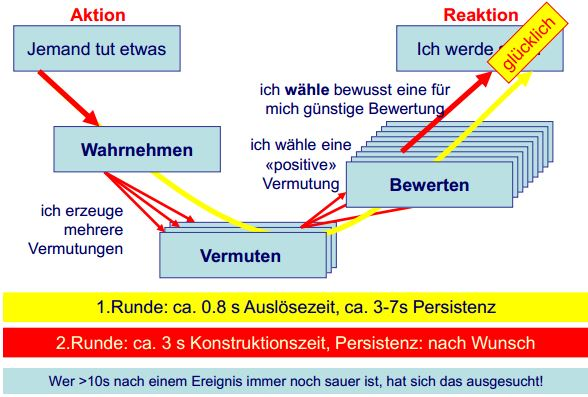
\includegraphics[width=0.7\linewidth]{fig/wahrnehmung-ablauf}
\caption{Wahrnehmungs-Ablauf}
\label{fig:wahrnehmung-ablauf}
\end{figure}

Wahr ist was ich zur Wahrheit bestimme. Gefühle basieren auf MEINER Realität.

\section{What we have learned}
Ich nehme die «Welt da draussen» nicht so wahr, wie sie ist, sondern wie sie mein Unterbewusstsein mir darstellt. Was ich bewusst wahrnehme, ist eine Mischung aus externer Realität, meinem Gedächtnis und meiner
Aufmerksamkeit. Mein Gedächtnis umfasst evolutionäre Erinnerungen und
eigene Lebenserfahrungen – gemischt mit vielem Anderen. Meine Gefühle und Reaktionen werden von meiner Wahrnehmung gesteuert: W-V-B => so fühle ich mich. Ich kann meine spontane Reaktion nicht verhindern, aber dann meine Gefühle selber steuern.

\section{INTEGRO}
Integro ist ein einfaches und praxiserprobtes Modell, um eine wichtige Dimension der Persönlichkeit zu verstehen: Stärken/Schwächen der Wahrnehmung und Eigenheiten der Kommunikation. Dies bezieht sich auf eigene sowie anderer Leute.

\paragraph{Hintergrund:} Menschen sind vielfältig und mehrdimensional, dies macht es schwierig sie zu verstehen. Ein vereinfachtes Modell hilft! Mit der Rückmeldung Anderer bekommt jeder ein klares Bild wie er auf andere wirkt. Wertungsfrei: Das Integro-Modell kennt keine guten oder schlechten Stile. Alle Stile haben ihre Stärken und Schwächen.

\begin{figure}[h!]
\centering
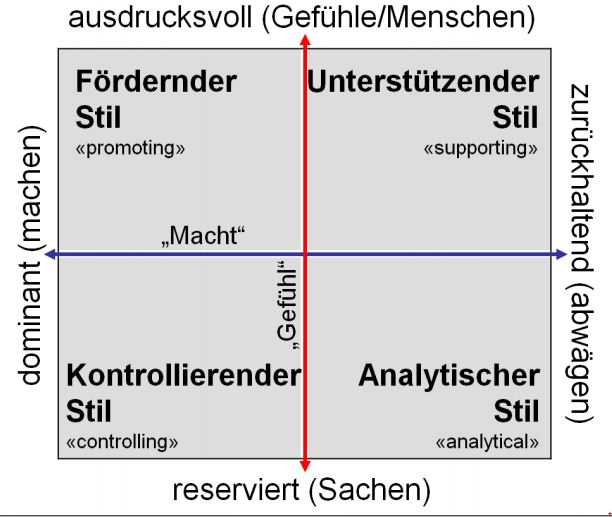
\includegraphics[width=0.5\linewidth]{fig/integro-modell}
\caption{Integro Modell [MEP]}
\label{fig:integro-modell}
\end{figure}

\begin{figure}[h!]
\centering
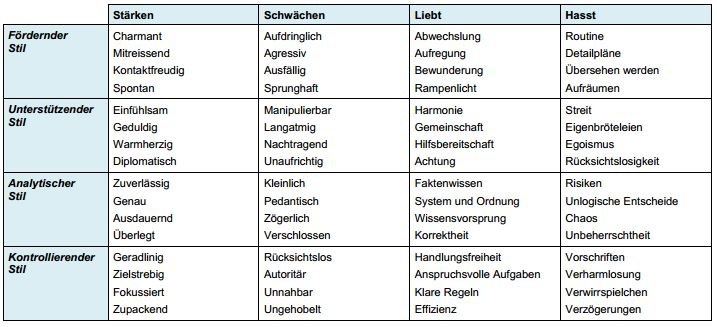
\includegraphics[width=0.7\linewidth]{fig/integro-uebersicht-stile-attribute}
\caption{Integro Übersicht Stile}
\label{fig:integro-uebersicht-stile-attribute}
\end{figure}

\subsection{Flexibilität}
Der eigene Stil ist langfristig stabil. Je nach Situation kann man auch andere Verhaltensweisen zeigen, wie leicht das gelingt zeigt die Flexibilität. Die Flexibiltät umfasst folgende Aspekte:
\begin{itemize}
	 \item die mittlere, allgemeine Neigung zu Flex- oder Inflexibilität
	 \item die momentane Flexibilität in der aktuellen Situation
	 \item die Leichtigkeit, vom stiltypischen Verhalten abzuweichen
	 \item die Reaktion auf Veränderungen und Überraschungen
\end{itemize}
Flexibilität kann man steuern und trainieren. Höhere Flex ist oft erwünscht.

\chapter{Präsentationstechnik}
Es ist wichtig, dass wir präsentieren können. Schlussendlich wollen wir immer unsere Lösung verkaufen. Wenn wir diese nicht präsentieren können, kauft diese auch niemand. Man muss \textbf{überzeugen}. Dabei spielt es keine wesentliche Rolle ob wir für einen, 12 oder 300 Zuhörer präsentieren.

\section{Vorgehensweise Präsentation vorbereiten (Grundsätze) [MEP]}
Nachfolgende Punkte dienen als Checkliste und können in dieser Reihenfolge abgearbeitet werden.

\begin{itemize}
	\item Aufgabenstellung klären (Briefing) \\
	Was ist das Thema? Ziel der Präsentation? Was ist der Anlass? Wer ist das Publikum? Was ist der Zeitrahmen? Welche Infrastruktur steht zur Verfügung?
	
	\item Material sammeln \\
	Wichtige Aspekte des Themas. Bilder, Zitate, Gegenstände, Handouts, Geschichten, Anekdoten, Versuchsergebnisse, Literatur. Bekannte Meinungen zum Thema. Gibt es Tabu-Zonen?
	
	\item Storyline entwickeln\\
	Man muss sich fragen wo das Publikum vor der Präsentation steht und wo man es nach der Präsentation haben will. Dient später als \textbf{Hilfsmittel}, der rote Faden, um das Publikum zu führen.
	
	\item Abschluss / Finale bestimmen\\
	Der letzte Eindruck bleibt am längsten. Vielleicht Bezug zum Titel der Präsentation, ein Film, eine Anekdote oder "die Moral der Geschichte ist ...", Metaphern. Musser aber zur Storyline passen!
	
	\item Einleitung / Aufhänger am Anfang bestimmen\\
	Interesse, Neugier, Aufmerksamkeit wecken. Teilnehmer positionieren! Frage ans Publikum, Bezug zum Titel, Facts, Geschichte ...\\
	Oft wird folgendes Muster empfohlen. Say, what you're gonna say. Say it. Say, what you have said. Dies wirkt aber oft ermüdend! Dies vorsichtig verwenden und nicht unnötige repetieren.
	
	\item Präsentationsmaterial ausarbeiten\\
	Auf Papier beginnen die Storyline zu entwickeln. Einteilung der Zeit (2-3 min pro inhaltliche Folie). Eventuell Handout machen. Schriftart und Schriftgrösse definieren.
	
\end{itemize}

\section{Merksatz}
\begin{itemize}
	\item Man muss nicht nur keine Idee haben, man muss auch unfähig sein, sie zu präsentieren.
	\item Es geht nicht darum, etwas zu sagen, sondern gehört zu werden!
\end{itemize}

\section{Eine Präsentation gut halten [MEP]}
\begin{itemize}
	\item Eine Präsentation ist ein Dialog (auch wenn es weitgehend schweigt).
	\item Der Teilnehmer will geführt werden.
	\item Halte das Publikum nicht für dümmer als es ist (Respekt und Ernsthaftigkeit ergibt Akzeptanz und Aufmerksamkeit).
	\item Nonverbale Signale der Teilnehmer beachten (Augenkontakt halten). 
	\item Störungen haben Vorrang (bei Störung hat der Vortrag keine Chance).
	\item Kämpfe nie gegen die Teilnehmer.
	\item Kenne Deinen Stoff!
\end{itemize}

\section{Tipps}
\begin{itemize}
	\item Vergleiche machen\\
	Wird beispielsweise mit grossen Zahlen gearbeitet, dann lohnt es sich ein gut vorstellbares Vergleichsmass zu nehmen. Bsp: 1 Bit = 1 Reiskorn, 1 CD = 750 MB = 180 T Reiskörner.
	\item Komplexe Strukturen (komplexe Organigramme)
	Eine komplexe Grafik kann nach und nach eingeblendet werden. Auf der ersten Folie nur die erste Hierarchie Stufe, auf der zweiten die nächste usw.
	\item Präsentation zu Hause trocken üben?\\
	Kann für ungeübte hilfreich sein um ein gutes Timing zu bekommen. Die Gefahr besteht, dass die Präsi dann nicht mehr so frisch sondern einstudiert wirkt.
	\item Folien überspringen?\\
	Oft ist es wichtig den Zeitrahmen einzuhalten und da kann es Sinn machen Folien zu überspringen. Zuvor muss man aber wissen welche und dazu vielleicht nur 1-2 Sätze sagen. Eventuell existiert dazu ein Handout.
	\item Animierte Folien verwenden?\\
	Komplexe Sachverhalte können oft nur gescheit mit Animationen präsentiert werden. Diese aber nicht als Spielerei missbrauchen!
	\item Inhalt der Folie vorlesen?\\
	Hängt vom Stil der Folie ab. Präsentationen sind keine Vorlesungen. Es gibt keine einheitliche Aussage dazu in der Praxis.
	\item Texte oder nur Stichworte?\\
	Zunehmend nur noch Bilder und Stichworte. Erfordert jedoch mehr Ausführlichkeit.
	\item Wie bereite ich mich auf eine wichtige Präsentation vor?\\
	Überraschungen vermeiden und Sicherheiten aufbauen. Redundante Infrastruktur, unsichere Technik vermeiden, Essen / Trinken / WC zuvor. Schöne und gemütliche Kleider. Inhalt kennen! Gelassenheit, Selbstvertrauen!
\end{itemize}



\chapter{Moderation \& Informelle Führung}

\section{Informelle Führung [MEP]}

\textbf{Führung} = Mit Leuten Ziele erreichen \\

\textbf{Formelle Führung} In einer Abteilung ist der Abteilungsleiter gegenüber den Mitarbeiter der disziplinarische Vorgesetzte. Er hat die organisatorische Befehlsgewalt.\\

\textbf{Informelle Führung} Wenn der Chef keine formelle Machtbefugnisse hat. Beispielsweise findet man dies in Projektteams mit Mitarbeitern aus verschiedenen Abteilungen. Informell führt man durch moderieren und teilnehmen - ohne Macht!\\

Der wichtigste Grundsatz für den informellen Führer im Umgang mit seinem Team ist folgender: Fragen statt Sagen! Wer fragt, führt - wer führt, gewinnt. Man muss seinem Team geistig voraus sein, sodass zum richtigen Zeitpunkt die richtigen Fragen gestellt werden.

\section{Teamwork}

\begin{itemize}
	\item jeder kommt gut vorbereitet
	\item jeder ordnet seine eigenen Interessen der Allgemeinheit unter
	\item es gibt keine Machtstrukturen
	\item jeder ist immer sachlich -- Gefühle haben im Geschäftsleben keinen Platz
	\item alle sind immer gut drauf, die Energie ist immer gleich hoch
	\item Konflikte lassen sich durch ein Gespräch unter 4 Augen bereinigen
\end{itemize}

\section{Ablauf einer Gruppen-Interaktion}

\begin{enumerate}
	\item Begrüssung durch Moderator
	\item Intro
		\begin{enumerate}
			\item Aufgabe, Ziel, erwartete Ergebnisse
			\item Ablauf
			\item Spielregeln
			\item Doku (Fotoprotokoll)
		\end{enumerate}
	\item Gruppenrunde (vorstellen)
	\item Informationsgleichstand herstellen
	\item Thema bearbeiten
	\item Handlungsorientierung (ToDo Liste)
	\item Abschluss (Offene Punkte, Feedback)
\end{enumerate}

\textbf{Bei einem Meeting sind folgende Punkt unerlässlich! [MEP]}
\begin{enumerate}
	\item Klares Ziel definieren, welche Ergebnisse müssen am Schluss vorliegen.
	\item Gruppenrunde ziemlich am Anfang des Meetings. Jeder sagt wenigsten einen Satz.
	\item Abschluss mit ToDo-Liste und kurze Feedback-Runde.
\end{enumerate}

\section{Drehbuch Workshop}

\begin{tabbing}
	\hspace{6cm}\=\kill
	\textbf{Start:} \> -- Mit Begrüssungskaffee/-tee beginnen (=Puffer) \\ \\
	\textbf{Gruppenrunde:} \> -- Immer! \\
						   \> -- Kann sehr kurz sein \\
						   \> -- Möglichkeiten: Steckbrief (Plakat/Folie), Gruppenspiegel usw. \\ \\
	\textbf{Mehrere Themen:} \> -- Liste machen \\ 
							\> -- gemeinsam Priorität bestimmen und Zeit vereinbaren \\
							\> -- Zeit überwachen, rückfragen ggf. Ziel anpassen \\ \\
	\textbf{Informations-Gleichstand:} \> -- Immer! \\ 
									   \> -- auch vor-verteilte Info kurz repetieren \\ \\
	\textbf{Themenspeicher:} \> -- Bei regelmässigen Meetings offene Themen festhalten \\ \\
	\textbf{Feedback:} \> -- Immer! \\
					   \> -- Zur Moderation, Zielerreichung, Arbeitsweise, usw. \\ \\
	\textbf{Pflicht-Plakate:} \> -- Spielregeln \\
							  \> -- Offene Punkte \\
							  \> -- Blitzlichtregeln
\end{tabbing}

\section{Meine Rolle als WS-Leiter}

Ich bereite den Arbeitsprozess der Gruppe methodisch vor und begleite ihn:
\begin{itemize}
	\item Drehbuch vorbereiten
	\item Umgebung gestalten
	\item Ergebnisse dokumentieren (Visualisieren, Fotoprotokoll)
\end{itemize}
Ich kümmere mich darum, dass die Gruppe (möglichst) immer am Punkt ihrer optimalen Leistungsfähigkeit arbeiten kann. Für das inhaltliche Ergebnis ist die Gruppe selbst verantwortlich!

\section{Workshop Spielregeln}

\begin{itemize}
	\item Jeder hier ist wichtig
	\item Kurz und Prägnant sprechen -- Zuhören und ausreden lassen
	\item Fragen statt interpretieren
	\item \emph{Ich} statt \emph{wir} oder \emph{man}
	\item Jeder ist für sich selbst verantwortlich
	\item Störungen haben Vorrang
\end{itemize}

\section{Vorbereitung eines Workshops}

\begin{tabbing}
	\hspace{3cm}\=\kill
	\textbf{Titel:}	\> -- Wenn nicht vom Auftraggeber definiert, selbst erfinden\\ 
					\> -- Keine Moderation ohne Titel!\\ \\
	\textbf{Zeitrahmen:} \> -- überprüfen, ob realistisch für die Zielerreichung mit einer Gruppe \\ \\
	\textbf{Ort:} 	\> -- Grosser Einfluss auf Gruppenenergie. Wird oft übersehen.\\ 
					\> -- Platz: 8-10 $m^2$/Person (bis ca. 10) \\ 
					\> -- ggf. Raum selber einrichten \\ \\ 
	\textbf{Ziel:} 	\> -- Zustand am Ende der Moderation aus der Absicht des Auftraggebers ableiten \\ 
					\> -- Erwartete Ergebnisse (auch negative Ziele) \\ \\
	\textbf{Teilnehmer:}	\> -- kann hierarchisch gemischt sein \\ 
							\> -- ggf.: Entscheidungsregeln klären \\ 
							\> -- einzeln durchbesprechen \\ 
							\> -- Anzahl: 8-12 = Optimum \\ 
							\> -- Bei grossen Gruppen: Teilgruppen! 
\end{tabbing}

\section{Was bedeutet Moderation?}

Moderation ist die bewusste Trennung von Prozessebene (wie gehen wir vor?) und Inhalt. Der Prozess, die Arbeitsmittel und -methoden sollten gruppenorientiert und ''gehirngerecht'' sein.

\section{Blitzlicht-Regeln}

Das Blitzlicht ist eine Technik, die mit wenig Vorbereitung und fast ohne Arbeitsmaterial durchgeführt werden kann. Während der Blitzlichtrunde äussern sich die Teilnehmer mit ein bis zwei Sätzen – nicht länger als eine Minute – zu einer vom Moderator gestellten Frage.

\begin{itemize}
	\item Jeder beantwortet die Frage für sich
	\item Keine Bezüge, keine Diskussionen
	\item Blitzlicht, kein Film
	\item Enden mit ''Punkt'' (z.B. der für mich wichtigste Punkt heute war...)
\end{itemize}

\section{Schlüssel-Elemente der Moderation}

\begin{enumerate}
	\item Setting (Halbkreis, keine Tische, Material)
	\item Themenneutrale Moderatoren
	\item Bewusste Trennung zwischen Prozess $\Longleftrightarrow$ Inhalt
	\item Fundierte Vorbereitung (durch Moderator)
	\item Visualisierung aller Ergebnisse
	\item Alle haben freien Zugang zum gemeinsamen Resultat
	\item Teilnehmer sind gleichrangig (können aber unterschiedlichen Einfluss haben)
	\item Klare Ziele, Spielregeln, Entscheidungsregeln
	\item Bewusstes Zeitmanagement
	\item Zweckmässige Umgebung
	\item Häufige Feedbackphasen
	\item Selbstverantwortung jedes Teilnehmers
\end{enumerate}

\chapter{Teamentwicklung}

\chapter{Selbstführung}
Führen von Menschen = mit Menschen Zielen erreichen. Man muss Menschen mögen. Die wichtigste Person, welche geführt werden muss, bin ich selbst. Dafür brauchts Selbsterkentniss, Selbst-Akzeptanz und Selbst-Steuerung.

Oft setzen wir uns eins Ziel (auf MEP lernen) und verhalten uns nicht zielführend (in Badi statt Lernen). Somit muss noch etwas anderes auf unseren Verstand Einfluss nehmen. 

\paragraph{Glaubensregeln}
Überlieferungen, kultureller Rahmen der Gesellschaft, eigene Lebenserfahrungen. Diese gehören zur Sammlung unserere Überzeugungen, welche wir unbewusst aufnehmen. Sind uns diese Regeln jedoch bewusst, können wir diese löschen, ändern oder ersetzen.

\section{Sie kennen die Bedeutung des Unterbewusstseins für unser Verhalten und wie man damit interagiert}

\paragraph{Erkentnisse zur Selbststeuerung}
\begin{itemize}
	\item Etwas mit dem rationalen Verstand zu wollen, genügt nicht zur wirksamen Zielerreichung
	\item Es gibt zwei relevante Akteure, die Einfluss auf mein Verhalten nehmen: Mein rationaler Verstand und mein Unterbewusstsein. (2 Optionen - Kampf gegen UB mit Disziplin und Verbissenheit oder Zusammenarbeit mit UB)
\end{itemize}

\begin{figure}[h!]
	\centering
	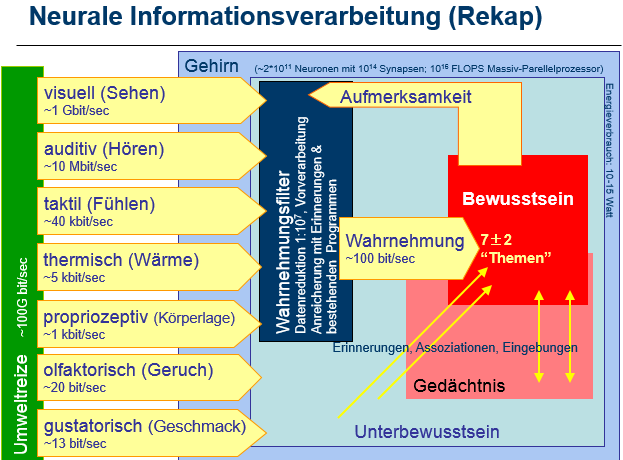
\includegraphics[width=0.7\linewidth]{fig/neurale-informationverarbeitung}
	\caption{}
	\label{fig:neurale-informationverarbeitung}
\end{figure}

Das Bewusstsein arbeitet lansgsam und nur unter guten Bedingungen. Es beobachtet und interpretiert (Pressesprecher des UB). Das UB reagiert schnell und in jeder Lebenslage. Beide arbeiten gleichzeitig und konkurrierend, sie können sich widersprechen. 

Erfolg = UB und Bewusstsein haben das selbe Ziel.

UB ist zu 100 Prozent ehrlich. Nimmt nie Rücksicht auf irgendetwas. Es ist fantasielos und nimmt alles wörtlich.

\paragraph{Steuerungsmöglichkeiten für das UB}
\begin{itemize}
	\item Gezielte Instruktion durch kluge Zielsetzung. Das UB hört mit. Durch gezielten Input kann ich die richtigen Programme im UB aufrufen.
	\item Re-Programmierung. UB funktioniert auf Basis gespeicherten Glaubenssätzen = kondensierte Erfahrungen = Programme. Ändern die Glaubenssätze, ändern die Programme dauerhaft! 
\end{itemize}

\paragraph{Wie programmiere ich das UB?}
Gut Frage Sherlock! Reden (einfach), Bild vorstellen (wirkungsvoll), körperlich erleben.

\paragraph{Wie weiss ich was das UB will? Wie es momentan programmiert ist?}
First of all - es kann nicht reden! Über Körperreaktionen, Gedankenblitzer, alle Sofortreaktionen.

\paragraph{Somatische Marker}
Jede körperliche Reaktion, jedes mentale Bild, Szene, Erinnerung. Die unmittelbare auf die Frage/den Begriff wahrnehmbar wird, ist ein somatischer Marker. Das emotionale Gewicht = Wert = +Lust/-Abscheu. Bsp: Kribbeln im Bauch, Erregung, Kneifen, plötzliche Schmerzen, Gefühl von Hunger/Durst usw.

\section{Sie wissen, welche Eigenschaften eine wirksame Zielformulierung umfasst}
\label{sec:how-to-be-successful-with-ub}

\begin{description}
	\item[1. Schritt - Satz was will ich] Ich gebe Instruktionen ans UB in Form von Sätzen, welche eine Zielformulierung beinhalten. Zielsatz formulieren, Zielsatz lesen. Welche Gefühle kommen dabei hoch? Somatische Marker +/- pro Wort bestimmen. Wenn weniger als -0/+70, Wort stärken.
	\item[2. Schritt - Motivation prüfen] 5 Gründe warum ich das Ziel erreichen will. Alle eigenen Gründe markieren, streichen aller fremden Gründe.
	\item[3. Schritt - Wirksamkeits-Check] Autonomie: Ich kann das Ziel selbständig erreichen. Wirksame Formulierung überprüfen (Erreichungsziel, keine Negation, keine Vergleiche, keine Relativierung, keine Zwänge, im Hier und Jetzt). Formulierung hat einen Energie-Pegel von -0/+70. 
\end{description}

Jetzt ist die Macht mit Dir! Das UB ist programmiert und unterstützt dich.
Nonplusultra: Das Ziel mit einer Metapher verknüpfen. Das UB arbeitet nun auch ohne meine Aufmerksamkeit.

\section{Sie wissen, wie ein Auftrag an das Unterbewusstsein (Programmierung) formuliert sein muss, damit es auch tatsächlich wie gewünscht wirkt.}

Siehe dazu \ref{sec:how-to-be-successful-with-ub}
	

\chapter{Project Setup \& Planning}

\section{Sie sind in der Lage, begründet darzulegen, worauf es bei dem Projekt-Setup ankommt.}

Ein Projekt ist ein zeitlich begrenztes Vorhaben mit einem definierten Anfang und Ende. Weil in den einzelnen Projektphasen viele Fragen auftauchen (Was ist das Problem?, Wie sehen die Prozesse aus? usw.), braucht es vor dem Projekt ein Projektsetup welche den Zeitrahmen, die Ziele und Resultate des Projektes festlegt.

\section{Sie können erläutern, was ein Projektziel ist und sind in der Lage, anhand einer Situationsbeschreibung korrekte Projektziele zu definieren.}

Projekt-Ziele beschreiben was man mit dem Projekt will. Folgende Fragen führen zu Projekt-Zielen:
\begin{itemize}
	\item Was soll erreicht werden?
	\item Welche Eigenschaften soll der Endzustand haben?
	\item Was ist nach dem Projekt anders - besser! - als vorher?
\end{itemize}
Projekt-Ziele sollten messbar und beurteilbar sein jedoch keine Lösung aufzeigen. Tipp: Zuerst Resultate beschreiben und danach die Ziele!

\section{Sie vermögen den Unterschied zwischen Projekt-Zielen und Projekt-Ergebnissen zu erklären.}

Von den Projekt-Zielen werden die Projekt-Ergebnissen/Resultate abgeleitet und von den Resultaten die einzelnen Arbeitspakete. Die Resultate sind die Ergebnisse die ein Projekt erzeugt. Resultate sind kein Aktivitäten (Nicht das Durchführen eines Workshops ist interessant, sondern z.B. die daraus hervorgegangenen Anforderungen.)

Ergebnisse in Softwareprojekten lassen sich fast immer in folgende Kategorien unterteilen:

\begin{enumerate}
	\item Applikationssoftware
	\item Applikationsdokumentation
	\item Prozesse
	\item Migration
	\item Rollout
	\item Projektmanagement-Ergebnisse
\end{enumerate}

\chapter{Fallstudie Project Planning}

In einer konkreten Fallstudie ging es um eine Planung eines Projekts, welche wie folgt gegliedert ist:
\begin{itemize}
	\item Geschäftsanalyse (Firma und Umfeld verstehen)
	\item Arbeitspakete (APs definieren und schätzen)
	\item Teamplanung (Teamzusammenstellung aufgrund von Profilen, Zuordnung von APs)
	\item Ressourcenplanung (Mitarbeiterplanung)
	\item Meilensteinplanung
\end{itemize}

\section{Geschäftsanalyse}
Bei der Analyse des Geschäfts müssen wir einmal mehr die Projektziele sowie die Anforderungen verstehen. Eine Anforderung ist eine Soll-Aussage über ein System oder einen Prozesse, welche eine Leistung oder eine Eigenschaft beschreibt. Anforderungen klar, einfach und messbar definieren. ''Antwortzeit des Dialogs in 97\% der Fälle unter 3 sec.''. Zielformulierungen und Anforderungen müssen demnach vorhanden sein.

\section{Arbeitspakete}
Mittels Anforderungen, Projektergebnisse und den Teilresultaten werden wir APs erstellen und die Aufwände für die APs schätzen.

\begin{itemize}
	\item Mapping aller Anforderungen zu den Resultaten. Damit keine Anforderungen vergessen gehen. Nebenbei können daraus die meisten APs definiert werden.
	\item Ein AP sollte in einer halben bis zwei Wochen abzuarbeiten sein und maximal 20 PT betragen. Somit brechen wir die Ergebnisse herunter. 
\end{itemize}

\subsection{Aufwandschätzung}
\label{sec:aufwandschaetzung}
In der Informatik unterschätzt man den Aufwand gerne! Also Achtung mit grosszügigen Schätzungen. Da sich ein Projekt im Laufe der Zeit ändert, muss man es auch kontrollieren. An folgenden Faktoren lässt sich schrauben, aber nicht unabhängig voneinander!

\begin{figure}[h!]
\centering
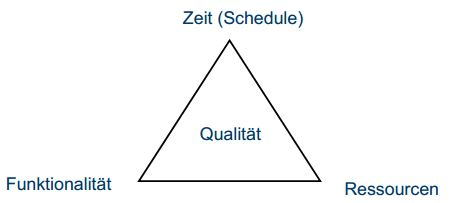
\includegraphics[width=0.3\linewidth]{fig/schaetzung-dreieck}
\caption{Schätzungs-Dreieck}
\label{fig:schaetzung-dreieck}
\end{figure}

Nachfolgend einige Schätzmethoden:
\begin{itemize}
	\item Individual Expert Judgmetn (WBS - Work Break Down Structure)
	\item Estimation by Analogy
	\item Count, Compute, Judge (Function Point Methode)
	\item Expert Judgment in Groups
	\item Formale Methoden
\end{itemize}

\paragraph{WBS} Projekt wird in APs unterteilt. Diese APs werden geschätzt. Diese ist am weitesten verbreitete Schätzmethode, oft sind es keine Schätzexperten und oft hat man keine Grundlage zum Schätzen. Kann erfolgreich sein, sollte aber nach Möglichkeit durch andere Methode ergänzt werden.

Best Practices: Projekt-durchführende Personen sollen schätzen. Tasks möglichst weit herunter brechen. Bei Unsicherheit bester und schlechtester Wert schätzen und Mittelwert nehmen. Alternativ kann auch eine Reserve von 10\% - 20\% hinzugezogen werden. Während dem Projekt aktuelle Resultate aufnehmen und vergleichen.

Wenn man die Implementation (inkl. Testing) schätzen muss, dann kann man im Normalfall den Wert fürs Design mal 2 rechnen.

Timeboxing bedeutet, dass der Zeitrahmen fix ist und der Scope vom Projekt angepasst werden darf.

\section{Ressourcenplanung}
\label{sec:ressourcenplanung}
Unter Ressourcenplanung verstehen wir die Zuordnung der Arbeitspakete zu den Projekt-Mitarbeiter und die Verteilung der Aufwände über die Zeit. Nachfolgende Aufzählung zeigt das Vorgehen bei der Ressourcenplanung:
\begin{enumerate}
	\item Festlegung der für die Arbeiten benötigten Profile und Zuordnung zu den Arbeitspaketen.
	\item Prüfen, welche Arbeitspakete parallel bearbeitet werden können. AP in Gruppen zusammenfassen. Alle AP einer Gruppe können parallel bearbeitet werden.
	\item 
	\begin{enumerate}
		\item Sichtung der verfügbaren Mitarbeiter und deren Profile und Zuordnung Mitarbeiter $\leftrightarrow$ Arbeitspaketen und ...
		\item Verteilung der Aufwände pro Arbeitspakete und Mitarbeiter auf die verfügbare Zeit und Beachtung der Auslastung der Mitarbeiter.
	\end{enumerate}
\end{enumerate}

\section{Meilensteinplanung}
\label{sec:meilensteinplanung}
Meilensteine sind wichtige Eckpunkte. Pro Meilenstein definiert man, welche Resultate erledigt sein müssen. Dies dient auch als Controlling-Punkt. Man kann genau sagen, wie weit der Projektfortschritt ist. Falls man nicht im Plan ist, kann man geeignete Massnahmen einleiten.

\section{Was ist der kritische Pfad in einem Projekt?}
Längster zeitlicher Pfad wo die Arbeitspakete hintereinander (seriell) gemacht werden müssen. Bestimmt wie lange das Projekt mindestens dauert.


\chapter{Projektrisiken}
Im Risikomanagement werden folgende Fragen geklärt:

\begin{itemize}
	\item Wohin läuft das Projekt?
	\item Welche Risiken und Unsicherheiten gibt es?
	\item Wie können diese beherrscht werden?
	\item Wie gehen wir mit sich ändernden Anforderungen um?
	\item Was müssen wir heute anders entscheiden, damit wir morgen mit unserem Projekt erfolgreich sind?
\end{itemize}

In vielen Unternehmen wird eine Kultur der Brandstifter gelebt. Es wird ein Brand gelegt, dieser wird unter grossen Einsatz gelöscht und dann wird man dafür ausgezeichnet. Besser ist aber eine Kultur in der Vorsorge belohnt wird.

\section{Sie können den Begriff des Risikos definieren und erläutern, mit welchen Methoden Risiken identifiziert werden können.}
\label{sec:risikomanagement-definition-risiko}

Ein Risiko ist ein unsicheres Ereignis mit negativen Auswirkungen. Risiko des Einen, Chance des Anderen. Kein Geschäftserfolg ohne Risiko. Risiken und Nutzen wachsen oft proportional.

\begin{center}
	\begin{math}
		Risiko = Eintrittswahrscheinlichkeit \times Auswirkung
	\end{math}
\end{center}

\paragraph{Vorgehen}
\begin{enumerate}
	\item Risiken identifizieren
	\item Risiken bewerten
	\item Risiken abschwächen
	\item Risiken verfolgen 
\end{enumerate}
Risiken können in die folgenden Arten unterteilt werden:
\begin{itemize}
	\item Technische Risiken
		\subitem Zu wenig Know-How zu einer Technologie
		\subitem Technische Spezifikationen von Produkten nicht korrekt
		\subitem Termintreue und Qualität von Lieferanten
		\subitem Patente von Mitbewerbern
	\item Implementierungsrisiken
		\subitem Anforderungen ändern sich oder Konflikte nicht aufgelöst
		\subitem Architektur \& Design falsch
		\subitem Entwicklungsprozess wird nicht beherrscht
	\item Wirtschaftliche \& Industrielle \& Geschäftsrisiken
		\subitem Ressourcen stehen nicht zur Verfügung
		\subitem Änderungen am Markt
		\subitem Mitbewerber haben bessere Produkte
		\subitem Verlust an kritischem Know-How durch Mitarbeiterfluktuation
\end{itemize}

\subsection{Identifzieren}
\begin{description}
	\item[Brainstorming] (immer) schnell, einfach, kann viele Risiken liefern. Jedoch systematische Fehler durch Gruppendruck, Vorurteile usw.
	\item[SWOT Analyse] (in komplexen Projekten) Projekt aus Sicht der übergeordneten Organisation betrachten. Stärken/Schwächen einer Organisation. Hilft, strategische Risiken zu identifizieren. Jedoch aufwendiger, ist der objektive Blickwinkel gegeben?
	\item[Bedrohungsszenarien] (bei konkreten Bedrohungen) Was wäre wenn? Situationen durchspielen, sind aber alle Situationen gefunden?
	\item[Übertragung von früheren Erfahrungen] (immer) Erfahrungen wiederverwenden. Aus Fehlern lernen. Konstruktive Analyse- und Lernbereitschaft vorhanden?
	\item[Interviews] (in komplexen Projekten) Identifikation von unklarer Schnittstellen und Erwartungen. Zeitaufwendig!
	\item[Konfliktanalyse] (bei konkreten Bedrohungen) Betrachtung von Interessensphären und Zielkonflikten. Beziehungen/Ziele von Schlüsselpersonen. Identifikation von WIN-WIN Situationen für Beteiligte. Anspruchsvoll, guter Kommunikationsstil nötig!
	\item[Checklisten] (immer) Erfahrungswesen aus der Literatur und der Branche. Einfach, Best Practices, geben Orientierung. Wie gut ist die Qualität der Liste?
	\item[Werkzeuge] Automatisierung systematischer Befragungen/Checklisten. Folgefragen in Abhängigkeit von Antworten. Automatische Auswertung. Nicht so einfach verfügbar!
\end{description}

Bei der Identifikation der Risiken fasst man diese in einer Tabelle zusammen. Man kann diese kategorisieren nach \textbf{Personen}, \textbf{Produkt}, \textbf{Prozess} und \textbf{Technologie}.

Top 5 der Risiken in Software-Projekten: 
\begin{enumerate}
	\item Ändernde Anforderungen
	\item Schlechte Benutzerschnittstelle
	\item Unzureichende Systemqualität
	\item Unrealistische Zeit- und Budgetplanung
	\item Technologieüberforderung oder unausgereifte Technologie
\end{enumerate}
	
\section{Sie kennen das Ziel und die wichtigsten Aufgaben des Risikomanagements.}

\paragraph{Ziele}
\begin{itemize}
	\item Potentielle Probleme erkennen bevor sie auftreten.
	\item Massnahmen ergreifen und durch gesamten Projektlebenszyklus durchführen, damit diese Probleme nicht auftreten und Projektziele gefährden.
	\item Risiken kontrollieren, nicht vermeiden.
	\item Frühzeitig und proaktiv an den Ursachen der wichtigsten Risiken eingreifen.
\end{itemize}

\paragraph{Aufgaben}
Siehe dazu die Liste Vorgehen in Abschnitt \ref{sec:risikomanagement-definition-risiko}


\section{Sie kennen Methoden zur Bewertung und Abschwächung von Risiken}

\subsection{Bewertung von Risiken}

Man muss das Risiko quantifizieren um diese vergleichen zu können. Die Risikobewertung sollte nie alleine durch Schlüsselpersonen wie der PL oder Projektowner erfolgen. Am besten zieht man sich ein externes Team hinzu. Oder von unabhängigen Gruppen identifizieren zu lassen. Zuerst ein Beispiel eines festgehaltenen Risikos:

\begin{table}[h!]
	\centering
	\begin{tabular}{|p{7cm}|p{7cm}|}
		\hline Risikoauslösendes Ereignis &  den Würfel werfen \\ 
		\hline Risiko & Geld verlieren, falls keine 6  \\ 
		\hline Eintrittswahrscheinlichkeit & 83 Prozent \\ 
		\hline Auswirkung & 10 CHF verloren \\ 
		\hline 
	\end{tabular}
\end{table}


Eine Möglichkeit ein Risiko zu schätzen ist die einfache Risiko Quantifizierung. Dabei geht es darum, jedem Risiko einen Zahl von 1-5 zu geben. Risiko mit dem Gewicht von 5 ist katastrophal und Risiko mit dem Gewicht von 1 ist vernachlässigbar. Zudem gibt es noch folgende Schätzmethoden:
\begin{itemize}
	\item Finanzielle Schätzmethoden: NPV und diskontierter Cash Flow (siehe Business Case)
	\item \textbf{PERT/Dreipunktschätzung: (w(pessim)) + 4 x w(realist) + w(optimist)) / 6}
	\item Machbarkeitsstudie
	\item ABC Analyse
	\item Delphi-Methode
	\item Expertenschätzung
\end{itemize}
Abbildung \ref{fig:risiko-management-beispiel-berechnung} zeigt wie das Risiko zusätzliche Tests einsetzen in einem Softwareprojekt bewertet wird.
\begin{figure}[h!]
\centering
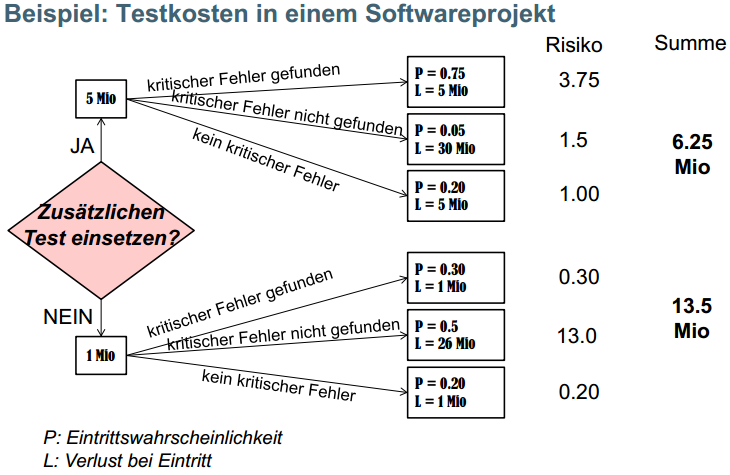
\includegraphics[width=0.7\linewidth]{fig/risiko-management-beispiel-berechnung}
\caption{Risikomgmt. Beispiel Berechnung}
\label{fig:risiko-management-beispiel-berechnung}
\end{figure}
Abbildung \ref{fig:risiko-management-muster-risiko-beschreibung} zeigt ein Muster für die Beschreibung eines Risikos.
\begin{figure}[h!]
\centering
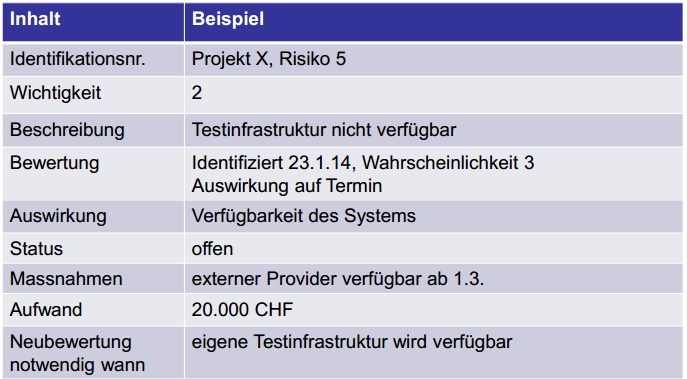
\includegraphics[width=0.8\linewidth]{fig/risiko-management-muster-risiko-beschreibung}
\caption{Risiko Management: Muster Risiko Beschreibung}
\label{fig:risiko-management-muster-risiko-beschreibung}
\end{figure}

\subsection{Abschwächung von Risiken}

Um ein Risiko abzuschwächen gibt es vier Möglichkeiten:
\begin{description}
	\item[Vermeiden] Eintrittswahrscheinlichkeit reduzieren. Man verzichtet so aber auch auf die Chance die das Risiko bietet.
	\item[Begrenzen] Auswirkung abschwächen. Wie bei einer Versicherung mit Selbstbeteiligung.
	\item[Behandeln] Durch zusätzlichen Aufwand Eintrittswahrscheinlichkeit und/oder Auswirkung reduzieren.
	\item[Ignorieren] Man lässt den Dingen seinen Lauf\dots
\end{description}
Abbildung \ref{fig:risiko-management-beispiel-abschwaechen-risiko} zeigt Massnahmen welche in den verschiedenen Kategorien ergriffen werden können um das Risiko abzuschwächen.
\begin{figure}[h!]
\centering
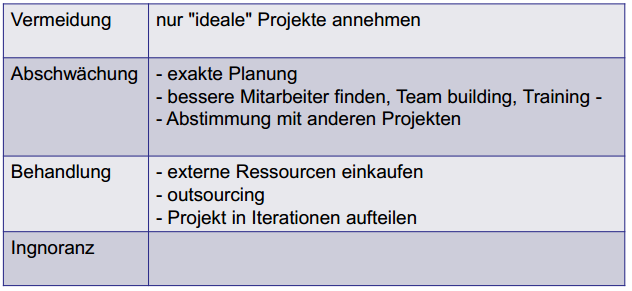
\includegraphics[width=0.7\linewidth]{fig/risiko-management-beispiel-abschwaechen-risiko}
\caption{Abschwächen des Risikos: Unzureichende Projektressourcen}
\label{fig:risiko-management-beispiel-abschwaechen-risiko}
\end{figure}
Risiken können auf mehreren Ebenen abgeschwächt werden:
\begin{description}
	\item[Innerhalb des Projekts] Frühzeitig sichtbare Risiken, die leicht abgeschwächt werden z.B. unklare Anforderungen, Fehler im Code usw. (Auf Ebene Meilenstein, AP).
	\item[Auf Projektebene] Spät sichtbare Risiken z.B. Integration von Komponenten, Abnahmen durch Kunden.
	\item[Für das gesamte Projekt] Sporadisch eintretende Risiken mit grösseren Auswirkungen z.B. Ressourcenmangel, Ausfall von Mitarbeitern.
\end{description}

Nach dem Risiken identifiziert, bewertet und abgeschwächt wurden, geht es darum, die Risiken auf dem Radar zu behalten. Nur Risiken die man aktiv verfolgt, verlieren Gefahrenpotential. Die vereinbarten Aktionen zur Abschwächung müssen überwacht werden. Greifen diese Aktionen zur Abschwächung? Hat sich die Bewertung geändert? Sind Risiken zu Probleme geworden? 

Bei mangelhaften Risikomgmt. entsteht oft folgendes: Feuerwehreinsätze (Risiken werden zu Problemen), unzufriedene Kunden (zu spät / zu teuer), teures Nacharbeiten, keine Systematik, keine Disziplin.
Abbildung \ref{fig:risiko-management-prozess} zeigt nochmal den gesamten Prozess des Risikomanagements zusammengefasst. Zudem ist auch die Kommunikation der Risiken (intern/extern) und die frühe Abschwächung (Projektstart) von Risiken wichtig.

\begin{figure}
\centering
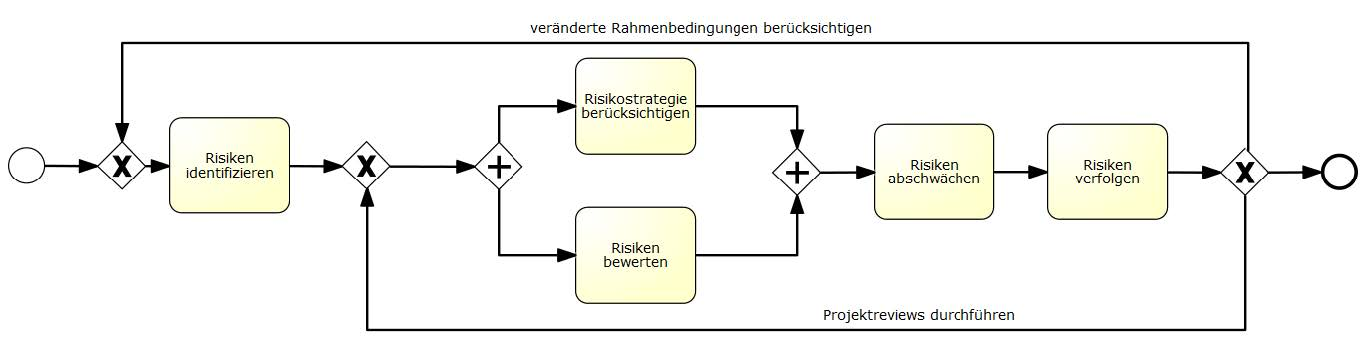
\includegraphics[width=0.7\linewidth]{fig/risiko-management-prozess}
\caption{Prozess des Risikomanagements}
\label{fig:risiko-management-prozess}
\end{figure}
 

\chapter{Projekt Controlling}

Vor dem eigentlichen Controlling muss der Projektplan (Ziel $\rightarrow$ Resultat $\rightarrow$ Teilresultat $\rightarrow$ Arbeitspaket) erstellt und die Arbeitspakete (zwischen 5-20 Personentage) geschätzt werden. Im Projektplan werden gleichzeitige APs zu Phasen zusammengefasst, welche sich an den Projektergebnissen orientieren. Für jedes Phasenende wird ein Meilenstein festgelegt. 
Liegt der Projektplan vor kann dieser regelmässig mit dem Ist-Zustand des Projektes verglichen werden. Dieser Abgleich nennt man Projektcontrolling. Das Projektcontrolling hat folgende Ziele:
\begin{itemize}
	\item Projekt in der Zeit und im Budget?
	\item Nächster Meilenstein erreichbar?
	\item Risiken frühzeitig erkennen und bei mehr Aufwand in einem AP Ressourcen verteilen
	\item Verbessern der Schätzungen durch ''Post Mortem'' Analyse.
\end{itemize}
Werden diese Ziele nicht erreicht muss etwas unternommen werden. Beim Projektcontrolling wird ein Soll-/Ist-Vergleich auf der Ebene der Arbeitspakete durchgeführt. Dabei wird jedes AP mit einer Status-Information (offen, in Arbeit, erledigt) versehen. Die Schätzung (SOLL) darf nicht mehr verändert werden. Zieht man das IST vom SOLL ab bleibt das Restbudget übrig (So viel dürfen wir noch verbrauchen...). Bei der Schätzung sollte man nie nach dem Fertigstellungsgrad fragen, sondern nach dem Restaufwand (RAS). SOLL - IST - RAS = positives oder negatives Gesamtergebnis. Kleinere Abweichungen können ausgehalten werden. Bei grösseren Aufwandserhöhungen müssen aber Ressourcen von andern AP umverteilt werden. Bei Software-Entwicklungsprojekten wird üblicherweise alle zwei Wochen ein Projektcontrolling durchgeführt. Bei längeren Projekten auch monatlich oder in kritischen Phasen auch wöchentlich.


\chapter{Organisatorische Projektführung}

Die organisatorische Projektführung besteht aus folgenden Elementen:
\begin{description}
	\item[Projektorganisation:] Festlegen der Organisation und Gremien in einem Projekt.
	\item[Rollen und Kompetenzen:] Festlegen der Rollen und deren Kompetenzen in einem Projekt z.B. IT- und Business Projektleiter.
	\item[Projektstruktur(plan):] Aufteilung eines Projektes in Teilprojekte oder Streams.
\end{description}

\section{Projektorganisation}
In der Abbildung \ref{fig:projekt-organisation} ist eine typische Projekt-Organisation abgebildet.

\begin{figure}[h!]
\centering
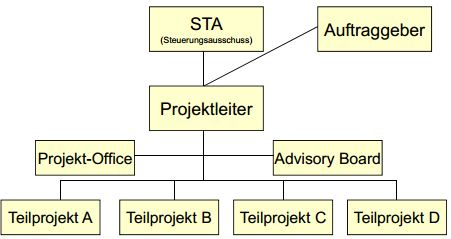
\includegraphics[width=0.7\linewidth]{fig/projekt-organisation}
\caption{Projekt-Organisation}
\label{fig:projekt-organisation}
\end{figure}

\section{Rollen}
Eine solche Organisation umfasst verschiedene Rollen:
\begin{description}
	\item[Projektleiter PL:] Führt und ''managed'' das Projekt. Jedes Projekt hat einen gesamtverantwortlichen Projektleiter. Verantwortlich für Resultate und erfolgreiche Durchführung.
	\item[Auftraggeber:] Der Sponsor überwacht das Projekt und trägt die volle Projektverantwortung, auch wenn er seine Aufgaben oder Kompetenzen teilweise delegiert (an PL oder STA).
	\item[Steuerungsausschuss (STA):] Kontrolliert und ''steuert'' das Projekt. Er gibt Budgets frei, nimmt Meilensteine ab oder entscheidet über die Weiterführung oder Abbruch. Unterstützt den Auftraggeber und tagt periodisch.
	\item[Teilprojektleiter:] Verantwortlich für ein klar abgegrenzter Teilbereich (Teilprojekt). Dieser hat für das Teilprojekt in etwa die gleichen Aufgaben und Kompetenzen wie ein Projektleiter.
	\item[Projekt-Office:] In jedem Projekt braucht es Sekretärinnen, welche administrative Aufgaben übernehmen. Es zählen folgende dazu: Meetings organisieren, Termine überwachen, Issuelisten führen, Kontrolle des Projektfortschritts.
	\item[Advisory Board:] Das Board besteht aus Experten, Schlüsselpersonen und Kunden des Projekts. Es ''berät'' das Projekt, gibt Feedbacks zu Lösungen und ist ein wichtiges Bindeglied zu den Benutzern. Es hat jedoch keine Entscheidungskompetenzen.
\end{description}

\section{Projektstrukturierung}
\label{sec:projektstrukturierung}
Eine Projektstrukturierung legt fest nach welchen Kriterien ein Projekt in Teilprojekte oder Streams unterteilt wird. Diese Struktur wird meist in einem Projektstrukturplan festgehalten. Folgendes sind Kriterien für eine Projektstrukturierung:
\begin{itemize}
	\item Grösse und Komplexität des Projektes
	\item Ausrichtung nach Resultaten oder Phasen
	\item Entkopplungsgrad der Teilprojekte und Parallelisierbarkeit der Arbeiten
	\item Zentralisierung oder Dezentralisierung von Verantwortung und Kompetenzen (Teilprojekte vs Streams)
	\item Geeignetes Personal: Verfügbarkeit von geeigneten TP-Leiter.
\end{itemize}

\subsection{Phasen- vs. ergebnisorientiert}
Wie in SoDa (Phasen \& Komponenten). Entweder strukturiert man das Projekt nach Phasen (Führung, Initialisierung, Konzeption, Realisierung, Einführung) oder nach Ergebnissen (Bsp: Weltreise - Transport, Übernachtung, Sehenswürdigkeiten, Verpflegung).

\subsection{Teilprojekte vs. Streams}
\begin{description}
	\item[Teilprojekt] Umfasst alle Elemente eines normalen Projekts. Ein TP-Leiter hat die volle Resultatverantwortung mit allen notwendigen Kompetenzen und Aufgaben wie Projektplanung, Budget, Controlling und Reporting.
	\item[Stream] Ein Stream ist ein Teilprojekt OHNE Resultatverantwortung und OHNE die klassischen Projektführungsaufgaben. Beides ist Aufgabe des PL!
\end{description}

\section{Lernziele}
\subsection{Sie kennen die Kriterien für die Definition einer Projektstruktur}
Siehe Abschnitt \ref{sec:projektstrukturierung}

\subsection{Sie können eine Projektstruktur definieren und begründen}
Siehe Abschnitt \ref{sec:projektstrukturierung}

\chapter{Kommunikation im Projekt}

\section{Sie kennen die Bedeutung und wichtigsten Elemente der Kommunikation im Projekt}

\subsection{Projektführungselemente}
\begin{description}
	\item[Interne]  Projektplanung (Resultate, AP, Aufwände, Meilensteine), Projektsitzung (Koordination, Abstimmung), TP-Review, Einzelgespräche / Stichproben.
	\item[Externe] Projektreport, Stakeholder-Management, Risiko-Management.
\end{description}

\subsection{Wichtigsten Fähigkeiten eines Projektleiters}
\begin{itemize}
	\item Leadership
	\item Kommunikation
	\item Problem-Lösung
	\item Verhandlung
	\item Beinflussung der Organisation (Organisational Change Mgmt.)
	\item Mentoring (Tutoren prädestiniert!)
	\item Prozess- and technische Expertise
\end{itemize}

\subsection{Wichtigsten Kommunikations-Werkzeuge}
\begin{description}
	\item[Projektsitzung] Kommunikation INNERHALB des Projekts.
	\item[Projektreport/-statusbericht] Regelmässige Kommunikation nach AUSSEN.
	\item[Stakeholder-Management] Gezielte Einflussnahme (Lobbying) auf Nutzniesser und Beteiligte bzw. Betroffene des Projekts.
\end{description}


\section{Sie sind in der Lage das Stakeholder Management zu erläutern ...}
Der Projektleiter kommuniziert mit Sponsoren, Projektteam, Kunden, Nutzern, Contractors und Lininenmanager.

\textbf{Stakeholder}: Anspruchgsruppe und -personen, die unmittelbaren Einfluss auf den Projektfortschritt haben und/oder von den Projektzielen direkt oder indirekt betroffen sind. Bsp: Finanzchef, Auftraggeber, Kunden, Gesetzgeber.

\noindent\fbox{%
	\parbox{\textwidth}{%
		Definition Stakeholder nach Chris Rupp: \textit{Ein Stakeholder eines Systems ist eine Person oder Organisation, die direkt oder indirekt Einfluss auf die Anforderung des betrachteten Systems hat.}
	}%
}
\\

Es gibt 4 Stakeholder-Gruppen:
\begin{description}
	\item [Promotoren, Sponsoren] aktive Unterstützuugn, Erfolg sicherstellen, Commitment, positive Energie, Macht, Geld, Ressourcen bereitstellen, bei Verlust schwerwiegende Folgen für Projektfortschritt
	\item [Supporters, Change Agents] inhaltliche Unterstützung, breite Abstützung in Organisation, punktuell Ressourcen bereitstellen.
	\item [Opponents, Change Barriers] Offene oder heimlicher Widerstand gegen das Projekt, wesentlicher negativer Einfluss auf Projektziele. Ziel: Projektabbruch, Umbesetzung von Schlüsselfunktionen, Aneignung des Projekts.
	\item [Hoppers, Change Advocates] unentschlossen, neutral, Stellung wechselnd, kein direkter Machteinfluss, aber Meinungsbildung möglich, durch Massnahmen => Supporters.
\end{description}

In einer Stakeholderanalyse müssen die Anspruchgsruppen identifiziert werden (\textbf{Stakeholderliste}). Die Einstellung derer zu den Zielen beurteilen (\textbf{Stakeholdermap} - wer kann mit wem und wie) und anschliessend Massnahmen erarbeiten (\textbf{Kommunikationsplan}).
	
Pro Stakeholder folgendes festhalten: Rolle, Name, Funktion, Auftrag, Ziele, Chance/Intressen, Risiken/Konfliktpotentiale und Massnahmen.


\section{... und eine Projektstandsitzung zu gestalten}
Wichtigstes Führungsinstrument innerhalb des Projekts. Die Agenda für eine Sitzung kann etwa so aussehen:

\begin{itemize}
	\item Letztes Protokoll (formale Abnahme)
	\item Allg. Infos (bswp. Organisatorische Veränderungen, Budgetpläne)
	\item Status u. Querinfos (Aktueller Stand der Resultate)
	\item Pendenzen
	\item Status der Issues (wichtige Fragestellungen aus dem Projekt)
	\item Risiken
	\item Nächste Termin
	\item Spezial und Fachthemen
	\item Ferienliste/Abwesenheiten
	\item Diverses
\end{itemize}

\textbf{Zweck} Regelmässige Informationsfluss innerhalb des Projekts. Übt einen gewissen Druck auf die Projekt-Mitarbeiter aus im Bezug auf die Resultate. Plattform um über Probleme zu sprechen, zu lösen und Entscheide zu fällen. Reporting der Projekt-MA und Teilprojektleiter gegenüber dem Projektleiter.

Agenda muss klar und fix sein. Wöchentlich oder 2x wöchentlich. Teilnehmer: Projektleiter, Teilprojektleiter oder Resultat-Verantwortliche. Dauer: max. 90-120 min.

\section{Sie können einen Projektreport gestalten und beurteilen}
Der Projektreport oder auch Projekt-Statusbericht dient als regelmässige Kommunikationsinstrument nach AUSSEN - gegenüber Auftraggeber, STC-Mitglieder, wichtigen Stakeholder, Kunde und Nutzer. Periode: Monatlich oder in intensiven Phasen wöchentlich möglich.

\subsection{Quellen}
Massnahmen-Katalog, Open Task Liste, Terminplan, Ressourcenplan, Lieferobjekte, Probleme, Risikokatalog, Projektkostenplan. Dies sind die Quellen für den Report, der PL ist darum besorgt die Quellen aktuell zu halten.

\subsection{Struktur u. Inhalt}
\begin{description}
	\item [Header] Berichtsperiode, Datum, PL, Autor
	\item [Projekt Status] Mit Ampeln arbeiten für die folgende Themen: Overall, Kosten, Zeit, Ressourcen, Focus und Interfaces. Zu jeder Ampel eine Info zusätzlich zu roten Ampel die Massnahmen. Man darf auch Erfolgsmeldungen melden.
	\item [Status Kosten] Soll-Ist
	\item [Status der Projektresultate] Next-Steps und Resultate Statis (Soll-Ist)
	\item [Risiken (optional)]
\end{description}


\chapter{Nutzenanalyse \& Business Case}

\chapter{Change Management im Projekt}
\label{sec:change_mgmt}

\section{Abgrenzung}
Wir behandeln nur Änderungen an \textbf{Projekt}anforderungen. Änderungen, welche keinen Bezug zum Projekt haben, wie Änderungen an \textbf{Produktiv}systemen gehören nicht dazu. Dies können bspw. Ergebnisse von Wartungsfällen, Erweiterungen oder Notfallmassnahmen nach Produktionsproblemen sein.

\section{Grundlagen}
Anforderungen ändern im Laufe der Zeit. Wir Menschen lernen dazu, Situationen ändern sich oder neue Gegebenheiten treten ein. Geänderte Anforderungen haben immer Auswirkung auf die Spezifikation. Sie können jedoch auch massive Auswirkung auf folgende Elemente haben:
\begin{itemize}
	\item Projektziel, Funktionalität des Zielsystems
	\item Architektur
	\item Projektdauer
	\item Projektkosten und Projektfolgekosten (Betrieb)
\end{itemize}

\textbf{Scope Creep} ist einer der häufigsten Gründe warum Projekte scheitern. In diesem Zusammenhang geraten die Anforderungen ausser Kontrolle, wenn unkontrollierte Änderungen zugelassen werden. Dies im Auge zu behalten ist daher sehr wichtig, besonders bei Festpreisprojekten.

Merksatz: \textit{''Wer alles reinlässt, kann nicht ganz dicht sein.''}. Unabgestimmte Änderungen am Projektrahmen (Spezifikation, Planung) sind absolut \textbf{verboten}.

\section{Ziele}
\begin{description}
	\item[Hemmschwelle] Bewusste Schwelle gegenüber unvermittelten Änderungen aufbauen. Jeder Änderungswunsch muss über die ''Latte''. So weiss jeder, dass man nicht einfach kommen kann und noch das und jenes ''gratis'' beantragen kann.
	\item[Angemessen behandeln] Änderungswünsche werden angemessen behandelt. Machbare Änderungen werden berücksichtigt, die Konsequenzen auf Scope, Budget und Zeit ist mit allen Betroffenen abgesprochen. Alle nicht machbaren Änderungen werden herausgehalten und am besten auch klar kommuniziert.
\end{description}

\section{Verfahren}
\label{sec:change_mgmt_verfahren}

\begin{itemize}
	\item Zu jedem Projekt gehören klare Festlegungen wie ein Change Requests abgewickelt wird.
	\item Solche Verfahren und die dazugehörigen Checklisten lassen sich in der Regel wiederverwenden.
\end{itemize}

Nachfolgen mögliche Checkliste bzw. ein Verfahren wie ein Change Management aufgesetzt werden könnte:
\begin{itemize}
	\item Es wird eine Gesamtliste aller beantragten CRs geführt einschliesslich Status jedes einzelnen CRs.
	\item Für jeden beantragten CR wird ein eigenes Dokument erstellt, in dem Folgendes festgehalten wird:
	\begin{itemize}
		\item Eindeutiger Identifikator des CRs
		\item Änderungshistorie des Dokuments
		\item Genaue Beschreibung der gewünschten Änderung. Hierzu gehören
		auch die Versionsnummern der betroffenen Dokumente, d. h. der
		Bezugspunkt für die beantragte Änderung!
		\item Machbarkeit (K. O.-Kriterium)
		\item Auswirkungen (Spezifikation und alle anderen betroffenen Dokumente, Aufwand (auch Gesamtprojekt), Kosten, Termine)
		\item Risiken
		\item Ziel-Release (wann soll der CR ausgeliefert werden?)
	\end{itemize}
	\item Festlegung, wer einen CR beantragen darf.
	\item Festlegung von Kriterien, wann ein CR vorliegt und wer entscheidet, ob ein CR vorliegt.
	\item Festlegung, wer über die Implementierung eines CRs entscheidet; die	Entscheidungsträger unterzeichnen dazu das CR-Formular.
	\item Die Annahme eines CRs führt zur konsequenten Änderung von Projektplan und Spezifikation, dann zur Implementierung.
	\item Gegebenenfalls Fristen für die Durchführung der einzelnen Schritte des CR Verfahrens (nicht zwingend).
\end{itemize}



\chapter{Strategische IT-Führung}

\begin{figure}[h!]
\centering
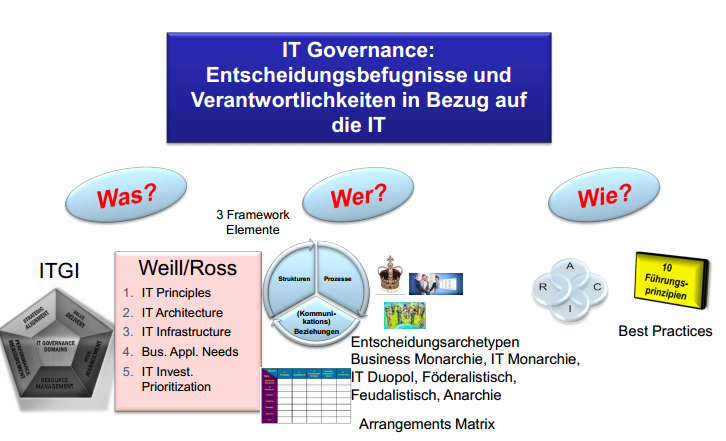
\includegraphics[width=0.8\linewidth]{fig/governance-big-picture}
\caption{IT Governance: Fasst alles zusammen, was man wissen muss.}
\label{fig:governance-big-picture}
\end{figure}

\section{Governance I}

\subsection{Begriff: IT Governance}
\textbf{Entscheidungsbefugnisse} und \textbf{Verantwortlichkeiten} in Bezug auf die IT.
\begin{quote}
	IT Governance specifies a framework for decision rights and accountability to encourage desirable behavior in the management and use of IT
\end{quote}


\subsection{Grundlegende Fragen zu Entscheidungen}
Diese Fragen, bzw. Elemente, müssen in einem Governance Rahmenwerk definiert werden.
\begin{description}
	\item[Was wird entschieden?] Governance Domains - Entscheidungsbereiche.
	\item[Wer entscheidet?] (Entscheidungsbefugniss)
	\item[Wie werden Entscheidungen umgesetzt?] Wie werden Entscheidungsfindungs-, ausführung und Verantwortlichkeiten implementiert.
\end{description}

\subsection{Differenzierung IT Management und IT Governance}
\paragraph{IT Management} Beschäftigt sich mit dem effizienten Betrieb der Unternehmens-IT. Software, Services, Infrastruktur, Projektdurchführung. Der Schwerpunkt liegt auf Administration Abläufe. Fokus auf interne Kunden. Stichwort \textbf{operativ}, Abteilungen und Individuen, Gegenwart, Kosten u. Qualität, Budgettreue, Durchführung.
\paragraph{IT Governance} Sichert, dass IT-Aktivitäten mit den aktuellen und zukünftigen Anforderungen des Business abgestimmt sind. Fokus auf interne und externe Kunden. Stichwort \textbf{strategisch}, Gesamtorganisation, Zukunft, Nutzen und Gewinn, sinnvolle Investitionen, Steuerung.

\subsection{Corporate Governance}
Umfasst die Strukturen und Prozesse zur Gesamtsteuerung des Unternehmens. Auf Ebene Verwaltungsrat und Geschäftsleitung. Im Mittelpunkt stehen Rechte und Interessen der Aktionäre und Teilhaber, Transparenz und Verantwortlichkeiten für die Entscheidungen.
Die Corporate Governance setzt somit Rahmen und Strukturen für die IT Governance.

\subsection{5 IT Governance Bereich (Domains) nach Weill/Ross}
\begin{description}
	\item[IT principles] Grundsätzliche Aussagen zum Stellenwert und zur Ausrichtung der IT. Basierend auf Geschäftsmodell. Welche Rolle spielt die IT? Entscheidender Wettbewerbsvorteil?
	\item[IT architecture] Regelt das Zusammenspiel zwischen Geschäftsarchitektur und IT Architektur. Stellt den Blueprint für die Integration, Entwicklung und Änderung der IT Assets zur Verfügung. Eine wohldefinierte, flexible EA ist eines der wichtigsten Governance Instrumente.
	\item[IT infrastruture] Strategie und Entscheide für die IT-Infrastruktur, die unternehmensübergreifend oder fachbereisübergreifend genutzt wird. Hardware, Software, IT Spezialisten. Angeboten als Services. Umfasst oft mehr als 50 Prozent der IT Kosten.
	\item[Business application needs] Wer definiert und genehmigt den Business Case. Definition der Projektverantwortung von den Requirements über Entwicklung zur Einführung. Wer entscheidet über die Architektur der Anwendung? EA-konform oder Innovationsausnahme?
	\item[IT investment prioritization] Wie viel und wo wird investiert? Durch welchen Prozess werden Projekte genehmigt? Wie erfolgt die Begründung eines Projekts? Projekt Portfolio Management?
\end{description}

\subsection{5 IT Governance Bereiche nach IT Governance Institute ITGI}
\begin{description}
	\item[Strategic alignment between Business and IT] Fortwährender Ausrichtung der IT an den Geschäftszielen und Geschäftsprozessanforderungen. Leistungen der IT in Art, Umfang und Qualität sind optimal auf die Bedürfnisse des Unternehmens ausgerichtet. Ziele für die IT sind klar definiert und von Businesszielen abgeleitet. Umsetzungsprozesse und –gremien exisitieren. IT Leistungen als Services verfügbar. Kontinuierliche Kommunikation zwischen Anbieter und Nutzer der IT Services. Investitionen klar am Unternehmensbedarf ausgerichtet.
	\item[Value delivery from IT to Business]. Wertbeitrag der IT ermitteln und stetig verbessern. Die IT von einer Unterstützungsfunktion zu einem Faktor der Wertschöpfung verändern. IT Dienstleistungen klar in Geschäftsprozesse integriert. Verwendung von Standards anstelle von proprietären	Individuallösungen. Überprüfung aller Prozessschritte und Aktivitäten auf Notwendigkeit und Wertbeitrag.
	\item[Management of the IT resources] Verantwortungsvoller und nachhaltiger Einsatz der Personal-, System- und Finanzressourcen. Ganzheitliche umfassende Betrachtung von Ressourcen und IT Prozessen. Prozesse sind standardisiert. Effiziente Gestaltung der IT Prozesse. Rollen und Verantwortlichkeiten sind klar definiert. Wissensmgmt. funktioniert.
	\item[Management of risks, security and rules] IT risiken identifizieren, richtig bewerten und angemessen behandeln. Risikotoleranz und Risikolevels sind für das Unternehmen definiert. Periodische Risikobewertung. Information Security Strategie existiert (abgenommen durch B. Hämmerli). Kosten proportional zum Wert eines IT Assets. 
	\item[Performance measurement] Transparenz der Leistungsstrukturen erhalten und Leistung messen und richtig beurteilen. Festlegung der Überwachung klar definierter Qualitätsmerkmale von IT Services. Regelmässiger Abgleich von Kennzahlen. Klar messbare Kennzahlen sind definiert.
\end{description}

\section{Governance II}
\subsection{RACI Modell}
\begin{description}
	\item[Accountable] Verantwortlich für Entscheidung.
	\item[Responsible] Verantwortlich für Durchführung.
	\item[Consulted] Wer wird in Entscheidungsfindung miteinbezogen.
	\item[Informed] Wer wird über den Verlauf oder zumindest über die Entscheidung informiert?
\end{description}
\subsection{Governance Entscheidungsarchetypen}
\subsubsection{Business Monarchie}
\textbf{Vorteile}
\begin{enumerate}
	\item Entscheidungen sind am Businessbedarf orientert
	\item Verantwortung des Business ist höher
	\item Schnelle Entscheidung
	\item Gute Umsetzungsunterstüzung vom Business
\end{enumerate}
\textbf{Nachteile}
\begin{enumerate}
	\item Zu wenig IT Knowhow
	\item Zu kurzfristig orientiert
	\item Zu kostenorientiert (zu wenig Investitionsbereit)
\end{enumerate}
\subsubsection{IT Monarchie}
\textbf{Vorteile}
\begin{enumerate}
	\item Technologisch gute Entscheidungen
	\item Auf IT Infrastruktur passende Lösungen
	\item Schnelle Trendserkennung
	\item Schnelle Entscheidung \& Umsetzung
\end{enumerate}
\textbf{Nachteile}
\begin{enumerate}
	\item Zu wenig kostenorientiert
	\item Technologieverliebte Entscheidungen, Einkauf unnötiger cooler Systeme
	\item Zu wenig Businessfokus, zu viel auf IT
\end{enumerate}
\subsubsection{Feudalistisch}
\textbf{Vorteile}
\begin{enumerate}
	\item Perfekt auf den Bereich zugeschnittene Lösungen
	\item Entscheidungen sind lokal verankert
	\item Schnelle Entscheidungen, da keine Abstimmung notwendig, keine Streitereien, jeder darf das haben was er haben will
	\item Hohe Dynamik
\end{enumerate}
\textbf{Nachteile}
\begin{enumerate}
	\item Heterogene Architektur
	\item Kostenintensive Integration
	\item Redundante Systeme
	\item Schlechter Informationsfluss
	\item Inseldenken
	\item Kaum übergreifende Lösungen -> IT Silos
	\item Kein Wissenstransfer
	\item KnowHow intensive IT
	\item Unternehmensweit unterschiedliches IT Wissen dass man nutzen muss
\end{enumerate}
\subsubsection{Föderalistisch}
\textbf{Vorteile}
\begin{enumerate}
	\item Breite Abstützung der Entscheidung
	\item Einheitliche Umsetzung ist einfacher
	\item Know How Transfer findet statt
	\item Hoher Meinungsaustausch, verschiedene Sichten, differenzierte Entscheidung möglich
\end{enumerate}
\textbf{Nachteile}
\begin{enumerate}
	\item Lange Entscheidungsprozesse
	\item Gefahr der Blockade einer Entscheidung - vorsichhenschieben der Entscheidung durch Grabenkämpfe, Krisen, gegenseitiges Blockieren...
	\item Teure Lösungen bei fehlenden Kompromissen
\end{enumerate}
\subsubsection{IT Duopol}
\textbf{Vorteile}
\begin{enumerate}
	\item Technisch und geschäftlich optimale Lösungen
	\item Transfer von Wissen zwischen Business \& IT
	\item Verbindung von Technologietrends \& Businessinnovation
	\item Gute Umsetzung
\end{enumerate}
\textbf{Nachteile}
\begin{enumerate}
	\item Verständnis \& Kommunikationsprobleme
	\item Gegenseitige Behinderung von Entscheidungen
\end{enumerate}
Unbedingt gemeinsame Ziele definieren!
\subsubsection{Anarchie}
\textbf{Vorteile}
\begin{enumerate}
	\item Sehr kurze Entscheidungsfristen (keine Absprachen nötig)
	\item Innovationsfreudig / Kreativ
\end{enumerate}
\textbf{Nachteile}
\begin{enumerate}
	\item Insellösungen / Adhoc Lösungen
	\item Heterogene IT Landschaften
	\item Hohe Wartungskosten
	\item Keine globale Strategie - grosse Investitionen sind nicht möglich
\end{enumerate}

\subsection{IT Governance Fallstricke}
\textbf{Symptome für Governance Probleme}
\begin{itemize}
	\item Bastellöusngen / SchattenIT
	\item Keine IT-Kennzahlen für Leistungsmessung / Bewertung de rIT
	\item Klagen über IT aus Management
	\item Redundante Systeme / Redundante Datenhalten
	\item IT entspricht nicht den Erwartungen
		\subitem Niedrige Kundenzufriedenheit
		\subitem Instabile Systeme
		\subitem Gescheiterte Projekte
	\item Explodierende IT Kosten bei niedrigem ROI
	\item IT Dienstleister nicht im Griff
\end{itemize}

\textbf{Massnahmen}
\begin{itemize}
	\item \textbf{Executive Engagement} \\
	IT Governance muss Chefsache werden
	\item \textbf{Policies as Strategic Tools} \\
		Es sollen klare und sinnvolle IT Prinzipien definiert werden, welche tatäschlich einen Nutzen bringen.
	\item \textbf{Defined Hierarchy of Governing Bodies} \\
		Wer was wie festlegen? Am besten eine Governence Arrangment Matrix aufbauen
	\item \textbf{Delegation of Authority and Precedent} \\
		Nicht zu viel zentralisieren bei den Entscheidungen, auch dezentrale Muster berücksichtigen.
	\item \textbf{Business Alignment} \\
		IT an Businessbedarf ausrichten
	\item \textbf{Proactive Liasion and Communications} \\
		Jeder Geschäftsbereich soll auf Management einen IT Ansprechspartner haben, der auch proaktiv auf sie zugeht und sie informiert.
	\item \textbf{Metrics and Reporting} \\
		Sinnvolle Kennzahlen definieren und erheben
	\item \textbf{Appropriate-Weight Procedures, Standards and Controls} \\
		Entscheidungen werden auf sinnvoller Ebene getroffen.
	\item \textbf{Independent Scrutiny} \\
		Das Reporting / Controlling wird von einer unabhängiger Instanz durchgeführt. Es geht nicht darum, die Leute zu überwachen, sondern um zu sehen ob es jetzt funktioniert.
	\item \textbf{Training and Awareness Program} \\
		Weiterbildung auf Governance Mechanismen
	\item \textbf{Easy-to-use Tools} \\
		Einfache Tools.
\end{itemize}

\chapter{Projekt Portfolio Management}

\section{Was verstehen wir unter (IT) Projekt Portfolio Management (PPM)?}

PPM legt systematisch und nachvollziehbar fest, welche Projekte in einem Planungszeitraum durchgeführt werden. Diese Projekte sollen die Unternehmensziele unterstützen und zusätzlich folgenden Kriterien gerecht werden:
\begin{itemize}
	\item Wirtschaftlichkeit (ROI)
	\item Beitrag zur Unternehmens- und IT-Strategie
	\item Projektrisiko (Realisierungswahrscheinlichkeit)
	\item Dringlichkeit
	\item Sicherheitsrelevanz
	\item Risikobereitschaft des Unternehmens
\end{itemize}

\section{Welche wesentlichen Aufgaben umfasst der PPM Prozess?}

\begin{enumerate}
	\item Bestandsaufnahme Projekte 
	\item Erfassung von Projektvorschlägen
	\item Bewertung der Vorschläge u.a. auf Basis Kosten, Nutzen, Risiko
	\item Portfolio-gestützte Auswahl anhand der definierten Kriterien
	\item Kommunikation der Entscheidungen
	\item Portfolio-Steuerung durch Projektcontrolling
\end{enumerate}

\section{Welche wesentlichen Gruppen von IT Aktiven können wir unterscheiden und wie verteilen sich die Investitionen auf diese?}

Es werden 4 Gruppen von IT Aktiven unterschieden. Die Prozentangabe ist der Anteil an den IT-Kosten in einem Unternehmen.
\begin{description}
	\item[Informationssysteme (13\%):] Alle Informationssysteme für die Entscheidungsfindung, Planung, Buchhaltung, Kontrolle, Kundenbeziehungen. Die Ziele dieser Gruppe sind präzisere Informationen und eine bessere Kontrolle was zu einer höheren Qualität führt. Mit dieser Gruppe können höhere Gewinnspannen und eine bessere Qualität erzielt werden. Die Bedeutung dieser Gruppe wächst durch mehr Bedrohungen und Risiken.
	\item[Strategische Systeme (13\%):] Eröffnen Eintritt in neue Märkte und ermöglichen neue Produkte oder Dienstleistungen. Das Ziel dieser Gruppe ist die Innovationssteigerung und Marktpositionierung was zu Wettbewerbsvorteilen und einem höherem Umsatz führt. Mit dieser Gruppe können höhere Produktpreise erzielt werden jedoch schlagen 50\% der Investitionen fehl.
	\item[Transaktionssysteme (27\%):] Automatisierung von Prozessen, Kostenreduktion, Volumenerhöhung. Die Ziele dieser Gruppe sind Kostenkontrolle und ein höheres Volumen. Mit dieser Gruppe ist eine Kostenreduktion und ein niedriges Projektrisiko möglich. Es werden auch immer mehr Berichte und Monitorings verlangt.
	\item[Infrastruktur (47\%):] Grundlage der allgemein verfügbaren IT Services, umfasst Technik und Menschen (Datenbanken, Netzwerke, Helpdesk usw.). Die Ziele dieser Gruppe sind eine Reduzierung der IT-Kosten durch Flexibilität und Standardisierung. Mit dieser Gruppe erzielt man eine niedrigere Gewinnspanne wohingegen der Marktwert des Unternehmens steigt. Es ist jedoch schwierig mit dem Kostendruck und den Technologieinnovationen mitzuhalten. 
\end{description}

\section{Nach welchen Kriterien werden IT Projekte häufig bewertet?}

IT Projekte werden grundsätzlich nach ihrem Nutzen (ROI), ihrer Realisierungswahrscheinlichkeit und ihrem Beitrag zur Unternehmensstrategie bewertet. Unternehmen können folgende IT-Portfolios definieren:
\begin{enumerate}
	\item Nutzen- und strategieorientiertes IT-Portfolio
	\item Nutzen- und risikoorientiertes IT-Portfolio
	\item Nutzen-, risiko- und strategieorientiertes IT-Portfolio
\end{enumerate}
Ein Unternehmen kann sich z.B. für ein Nutzen- und strategieorientiertes IT-Portfolio entscheiden. Dabei wird der ROI des Projektes untersucht und welchen Beitrag das Projekt zur Unternehmensstrategie liefert. Aufgrund dessen wird entschieden ob das Projekt durchgeführt oder abgebrochen (verschoben) wird.
Abbildung \ref{fig:bewertung-it-projekt} zeigt eine Übersicht über die Kriterien nach welchen ein IT-Projekt bewertet werden.

\begin{figure}
\centering
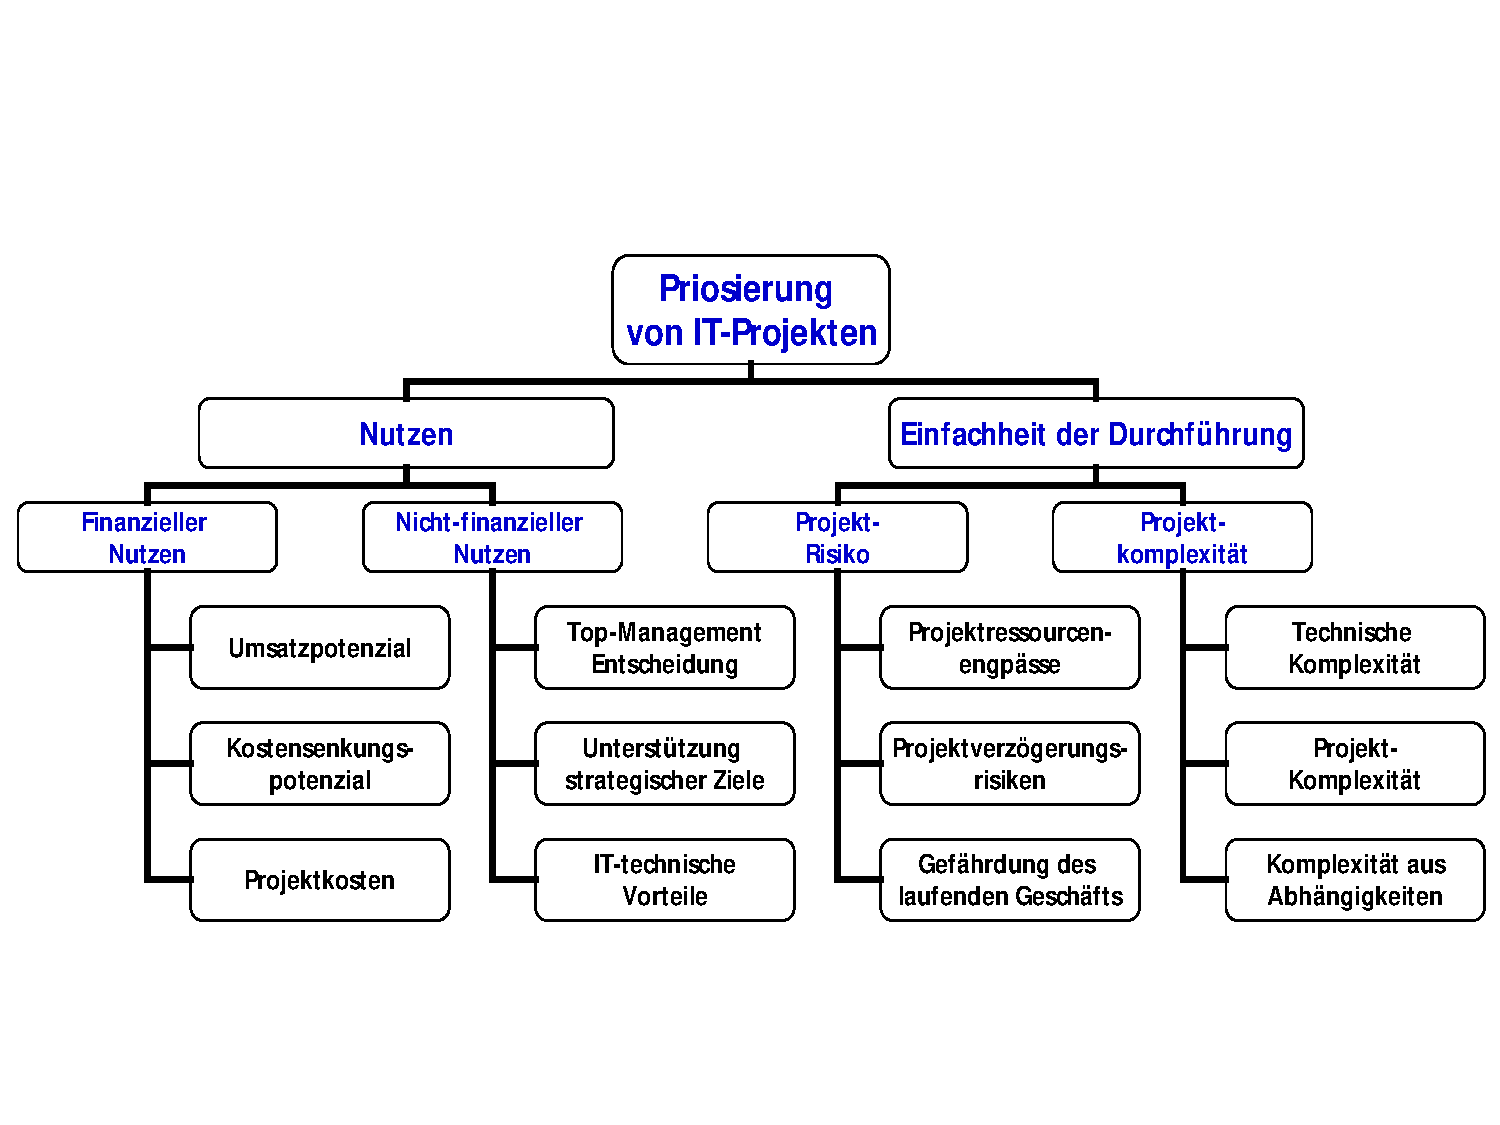
\includegraphics[width=\linewidth]{fig/bewertung-it-projekt}
\caption{Bewertungskriterien von IT-Projekten}
\label{fig:bewertung-it-projekt}
\end{figure}

\section{Nennen Sie Beispiele für typische Fehler im PPM.}

\begin{enumerate}
	\item PPM ist nicht an die Bedürfnisse des Unternehmens angepasst und ist nicht akzeptiert
	\item Zu schwerfällige Prozesse verhindern Innovation
	\item Projektberichte führen nicht zu Entscheidungen
	\item Kein Abbruch von scheiternden Projekten (Abbruch schafft Ressourcen für starke Projekte)
	\item Fehlerhafte Projektdaten (Schätzungen verbessern durch Abgleich mit Ergebnissen)
	\item Keine rechtzeitige Anpassungen der Projektziele
	\item Keine Bereitstellung der benötigten Ressourcen (Genehmigte Projekt müssen ihre Ressourcen kriegen)
	\item Unzureichende Projektplanung
\end{enumerate}

\section{Nennen Sie Beispiele für Standards, die zur Definition eines Unternehmens PPM konsultiert werden können.}

\begin{description}
	\item[IT Infrastructure Library (ITIL):] Gute Quelle für Metriken und Verständnis von Best Practices für IT Strukturen und Prozesse.
	\item[Control Objectives for Information and related Technology (COBIT):] Controlling-Instrumentarium im Rahmen der ITGovernance. 
	\item ISO 38500 (Norm für IT Governance)
\end{description}}

\chapter{IT Trends}
\section{Grundbegriffe zu Trends}
\subsection{Begriffsdefinition}
Der Begriff \textit{trend} stammt aus dem Englischen \textit{to trend}, was so viel bedetet wie \textit{in bestimmte  Richtung verlaufen}. Generell ist es eine Veränderung in der Gesellschaft / Wirtschaft oder Technik, welche eine neue Bewegung oder Richtung auslöst.
\subsection{Trend als Extrapolation}
Ein Trend kann man gut beobachten, aber schlecht messen. Man nimmt dazu bereits bekannte Daten, analysiert die und versucht, eine Aussage über den Verlauf in der Zukunft zu treffen. Typischerweise kann man den Trend selbst nicht beeinflussen. Dabei trifft man auch auf das Problem der sich selbst erfüllenden Prophezeiung - wenn man sagt, dass Firma X in den nächsten Jahren sehr stark sein wird, so ist das Vertrauen in die Firma grösser und die Wahrscheinlichkeit höher, dass sie tatsächlich sehr stark sein wird.
\begin{figure}
\centering
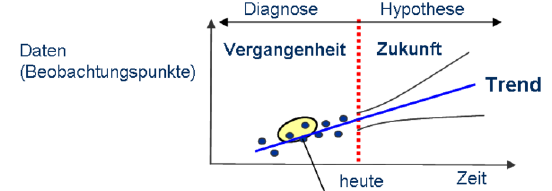
\includegraphics[width=0.7\linewidth]{fig/trend}
\caption{Anatomie eines Trends}
\label{fig:trend}
\end{figure}
\subsection{Quellen}
Trends werden z.B. von Business Analysten und Beratungsfirmen, aber auch von den Technologie Unternehmen selbst publiziert. Die Technologie Unternehmen publizieren diese, da sie ihre Innovationskraft demonstrieren möchten, verwenden es also als \textbf{Marketinginstrument}. Die Business Analysten  / Beratungsfirmen verdienen damit ihre Brötchen!
\subsection{Faktoren die zu Trends führen}
Oder einfach Faktoren, welche unsere Zukunft mitbestimmen. Diese sind extrem vielfältig, und haben 5 Kernpunkte;
\begin{enumerate}
	\item Gesellschaft
	\item Biosphäre
	\item Technologie
	\item Politik
	\item Wirtschaft
\end{enumerate}
Diese Kernpunkte beeinflussen sich alle gegenseitig.
\subsection{Trenddarstellungen}
Es gibt verschiedene Wege, wie man einen aktuellen / vergangenen Trend darstellen kann. Diese sind nachfolgend vorgestellt.
\subsubsection{Hypekurve}
\begin{figure}
\centering
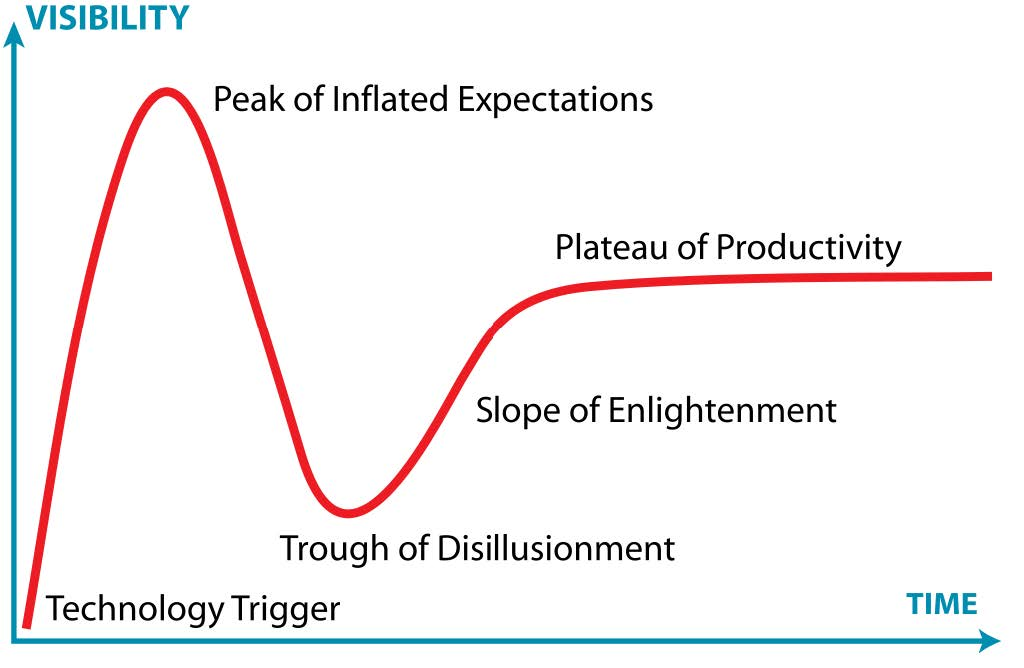
\includegraphics[width=0.7\linewidth]{fig/hype_kurve}
\caption{Die Hypekurve}
\label{fig:hype_kurve}
\end{figure}
Die Hypekurve beschreibt folgendes Phänomen: Am Anfang ist die Technologie noch unbekannt, deswegen am Boden. Danach wird die Technologie entdeckt und überall gross in den Medien präsentiert, wobei natürlich grosse Erwartungen in die Technologie gesteckt werden. Danach sinkt das Interesse relativ schnell, da die Erwartungen nicht erfüllt werden konnten. Später, wenn das \textit{wahre} Potenzial der Technologie erkannt wurde, steigt die Visibliät nochmals und bleibt stabil. \\
Der Nachteil an dieser Darstellung ist, dass sie gar keine Vorhersagekraft besitzt, sondern nur den aktuellen Stand kommentiert. Zudem entbehrt sie jeglichen wissenschaftlichen Grundlagen und missachtet den Fakt, dass ein Top oder Flop nicht nur von der Technologie abhängig ist, und es durchaus möglich ist, dass eine Technologie auch einfach verschwindet, ohne je das \textit{Plateau of Productivity} erreicht zu haben.
\subsubsection{Trendliste}
Eine einfache Liste, was denn im Moment am Aufstreben ist. Lässt sich über die Jahre vergleichen - war dieser Trend tatsächlich richtig?
\subsubsection{Trendwellen}
Trends treten in Wellenform auf - leider verstehe ich das nicht und im Internet tritt diese Grafik extrem selten auf...
Reviewer - Entscheide ob du obs rein gehört oder raus muss.
\begin{figure}
\centering
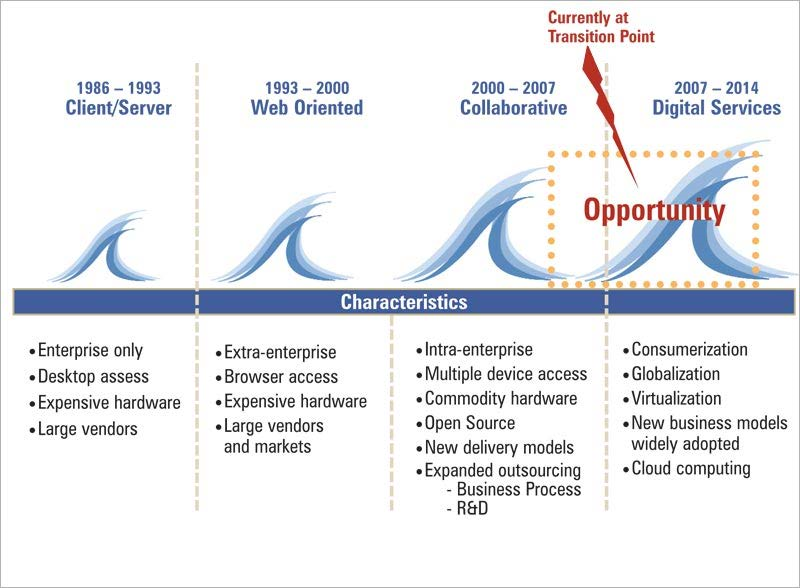
\includegraphics[width=0.7\linewidth]{fig/waves}
\caption{}
\label{fig:waves}
\end{figure}

\section{Trendkritik, Spekulationen, Kontroversen}
\subsection{Hardware vs Fähigkeit}
Nur weil man eine Videokamera und einen PC hat, heisst das noch lange nicht dass man damit einen Kinofilm herstellen kann. Das heisst, dass wir heute zwar aus der Perspektive der Rechenleistung die Möglichkeit haben, einen Menschen zu simulieren, praktisch aber die Fähigkeit dazu (noch?) nicht haben.
\subsection{Wie gut ist eine Trendanalyse?}
Dies kann man anhand folgender Faktoren bewerten:
\begin{enumerate}
	\item Qualität der Daten (z.B. Umfang der Stichproben)
	\item Unabhängigkeit/Interessen der Analysenhersteller
	\item Wie weit voraus gehen die Prognosen?
	\item Art der Aussagen in der Analyse
	\item Sind andere derselben Meinungen? Gibt es andere, zusammenhängende Trends?
\end{enumerate}

\section{Vergangene und aktuelle Trends}
\subsection{Vergangene Trends}
\begin{enumerate}
	\item \textbf{Moore's Law} \\
		Anzahl der Transistoren pro Fläche verdoppelt sich alle 12 Monate (oder 18 oder 24).
	\item \textbf{Smartphones}
	\item \textbf{Soziale Netzwerke}
	\item \textbf{VoIP}
	\item \textbf{LEDs}
	\item \textbf{...}
\end{enumerate}
Es zeigt sich, dass auch Gartner (deren Kerngeschäft es ist, Aussagen über Trends zu treffen), oftmals nicht ganz so richtig liegen wie sie das gerne hätten, auch wenn es nur um Prognosen für die nächsten 2/3 Jahre geht. So sagten sie beispielweise, dass 2015 25\% der Arbeitsstunden beim Betrieb von IT Services durch den Einsatz von Automationstools eingespart werden.
\subsection{Aktuelle Trends (2015)}
\begin{enumerate}
	\item Computing Everywhere
	\item Internet of Things
	\item 3D Printing
	\item Advanced, Pervasice and Invisible Analytics
	\item Context-Rich Systems
	\item Smart Machines
	\item Cloud/Client Computing
	\item Software Defined Applications \& Infrastructure
	\item Web-Scale IT
	\item Risk-Based Security and Self-Protection
\end{enumerate}

\section{Cloud \& Big Data Trends umsetzen}
\subsection{Definition}
Jetzt hat jedes Fach eine Definition von Cloud, die hier kommt vom National Institute of Standards and Technology, also  vertrauenswürdiger als Chip Online...
\textit{A model for enabling ubiquitous, convenient, on-demand network access to a shared pool of configurable computing resources (e.g. networks, servers, storage, applications, and services) that can be rapidly provisioned and released with minimal management effort or service provider interaction.}
\subsection{Merkmale}
Auch hier...
\begin{enumerate}
	\item \textbf{Leistung nach Bedarf}
	\item \textbf{Abrechnung nach Nutzung}
	\item xyz as a Service
	\item Verteilt und mehrfach genutzt
	\item Internet Technologie basiert
\end{enumerate}
Klar, es gibt SaaS, PaaS und IaaS, kennen wir aus SSM.
\subsection{Warum Cloud?}
Ich wiederhole mich, wenn ich sage, dass sich das hier wiederholt. Tue aber ich, und das hier tut es auch. Yo dawg I heard you like repeations.
\begin{enumerate}
	\item Schnelle Reaktion auf Veränderungen
	\item Niedrigere Fixkosten \& Transparenz in den Kosten
	\item Fokus auf Kerngeschäft
	\item Weniger Know-How zum Betrieb notwendig
	\item Know-How der Anbieter zum eigenen Vorteil nutzen (Neue Technologien \& Referenzarchitekturen)
\end{enumerate}
\subsection{Warum nicht Cloud}
\begin{enumerate}
	\item Werden Standards in der Cloud beachtet? Kann ich einfach wieder weg?
	\item Wie stabil ist mein Anbieter?
	\item Habe ich die Kontrolle über meine Daten noch?
	\item Muss ich mir neue Skills aneignen, um die Cloud effektiv nutzen zu können?
	\item Wie sieht es mit der Cloud Governance aus?
\end{enumerate}
\subsection{Governance in der Cloud}
\begin{enumerate}
\item Wer im Unternehmen kauft externe Cloud Services ein?
\item Sind die Einkäufer juristische Vertreter des Unternehmens?
\item Wer prüft die Verträge?
\item Welches Recht kommt zur Anwendung bei Problemen?
\item Welches Preismodell ist gut für Ihr Unternehmen?
\item Wo sind die Daten und wie steht es um Datenschutz und Zugriff?
\item Wieviel Zeit bleibt, wenn sich ein Cloudservice ändert?
\item Wieviel Zeit haben Sie, wenn der Service verschwindet?
\item Was ist zu tun, wenn Sie den Cloudanbieter wechseln wollen? Geht es überhaupt? Wieviel wird es kosten?
\item Welche Informationswege, Entscheidungsprozesse, Eskalationsmechanismen bestehen mit dem Cloudanbieter?
\item Wie sichern Sie Transparenz?
\item Was heisst Backup in der Cloud?
\item Haben Sie den Zugriff auf alle Informationen, um Berichtspflichten und Audits erfüllen zu können?
\item Wissen Sie, welche anderen Cloudanbieter Ihr Vertragspartner involviert hat?
\item Wer haftet für Schäden?
\end{enumerate}
\subsection{Mögliche Strategie für den Wechsel in die Cloud}
DoD = Department of Defense (USA)
\begin{figure}
\centering
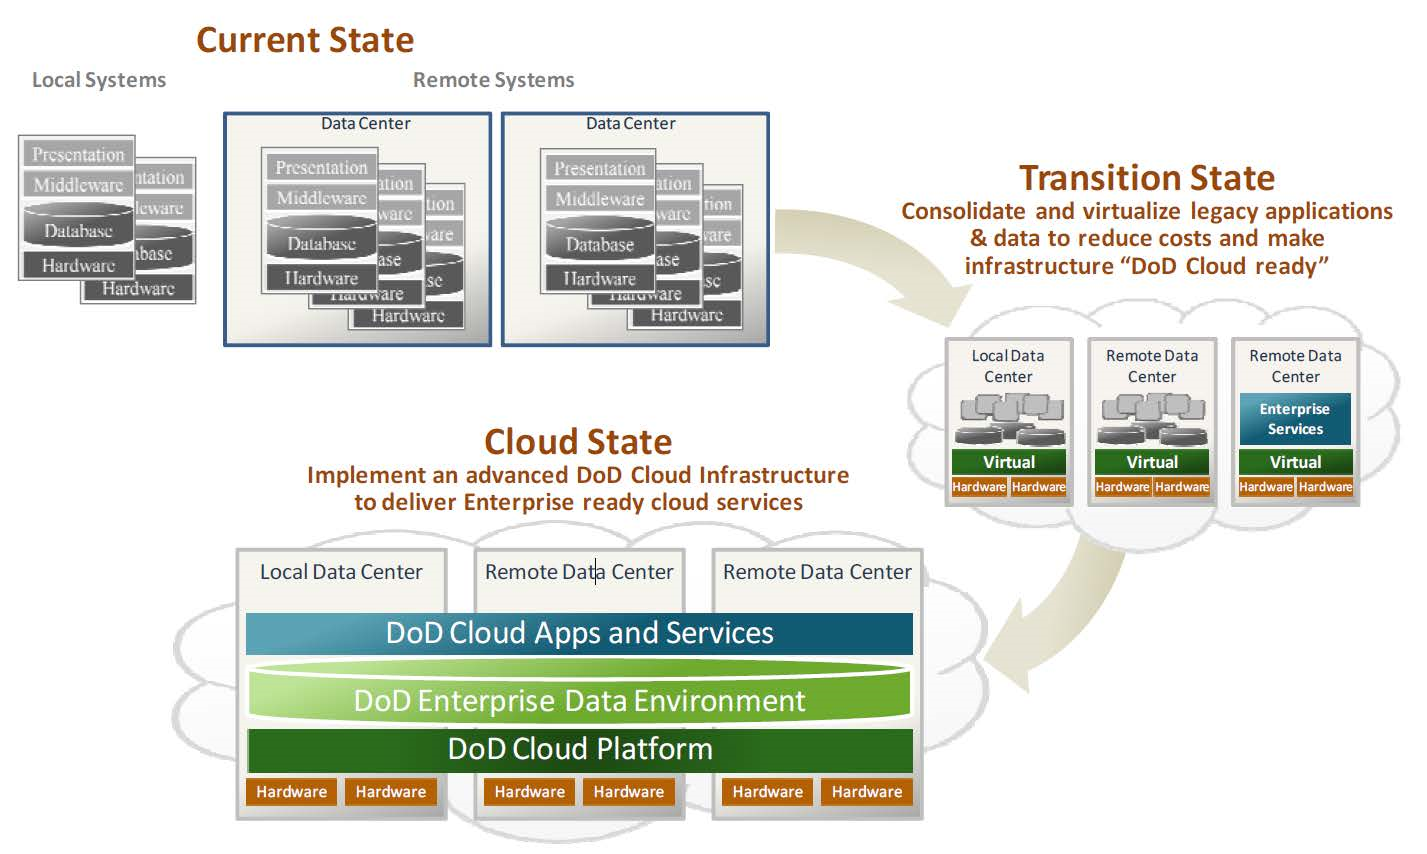
\includegraphics[width=0.7\linewidth]{fig/dod_cloud_transition}
\caption{Department of Defense Cloud Transition}
\label{fig:dod_cloud_transition}
\end{figure}
Zuerst haben wir überall unsere Applikations-Silos, mit eigener Hardware, eigenen Datenbanken \& Middleware, ... Das brechen wir im \textit{Transition State} auf, und virtualisieren die ganze Chose zuerst einmal, wobei wir auch Enterprise Services von extern implementieren. Zum Schluss haben wir eine homogene Umgebung, welche komplett in der Cloud und auf Service-Basis funktioniert.\\
Allgemein sollten bei der Implementierung von Cloud Services zuerst die SaaS-Angebote geprüft werden, und möglichst viel davon sollte daraus abgedeckt werden. Danach PaaS und zuletzt IaaS.
\subsection{Cloud Typen}
Hier gibt es lustige Arten von Cloud.
\subsubsection{On-Site Private Cloud}
Die Cloud, welche bei der Firma im Keller unten steht. Dabei hat natürlich die Firma Zugriff auf die Ressourcen.
\subsubsection{Outsourced Private Cloud}
Dabei hat man eine eigene Umgebung bei einem externen Anbieter. Also wenn z.B. die Swisscom eigens eine OpenStack Umgebung für einen aufbaut und betreibt. Hier hat auch nur die Firma, welche den Auftrag für die Cloud gegeben hat, den Zugriff auf die Ressourcen.
\subsubsection{Community Cloud}
Eine \textit{Community Cloud} dient mehreren Nutzern, welche gemeinsame Interessen haben, nicht nur einer einzelnen Firma. Dies kann z.B. Switch Drive sein, welche ja allen Studenten / Universitätsmitarbeitenden zur Verfügung steht. On-Site bedeutet hier, dass die Nutzer die Cloud selbst betreiben Outsourced wäre, wenn sie diese auch extern geben.
\subsubsection{Public Cloud}
Public Cloud ist klar, Services, welche allen Nutzern zur Verfügung stehen, betrieben von z.B. Amazon.
\section{Big Data}
\subsection{Definition}
By Gartner! Not Chip Online!
\textit{“Big data” is high-volume, -velocity and -variety information assets that demand cost-effective, innovative forms of information processing for enhanced insight and decision making.}
\subsection{4 V's}
Grüsse aus DMG
\begin{enumerate}
	\item \textbf{Volume} Grosse Menge an Informationen
	\item \textbf{Variety} Unterschiedlichste Formate der Informationen
	\item \textbf{Velocity} Zeitkritisches Auftreten - Morgen schon wieder unnütz.
	\item \textbf{Veracity} (unklare Qualität der Daten)
\end{enumerate}
\subsection{Nutzen von Big Data}
\begin{enumerate}
	\item Informationen schneller transparent und nutzbar machen
	\item Präzision der Informationen erhöhen
	\item Nutzung von daten für Szeniaren Analysen \& Vorhersagen
	\item Anlayse der Kunden und individuelle Lösungen für Kunden
	\item Verbesserte Entscheidungen
	\item Neue Produkte und Services (z.B. Facebook kann Katzenfutter-Werbung an jmd schalten, der häufig Katzenvideos hochlädt)
\end{enumerate}
\subsection{Big Data in der Praxis}
Richtig grosse Datenmengen à la Facebook trifft man in der Praxis eher selten an. Also im kleinen anfangen! Das sog. \textit{Compley Event Processing / Social Analytics} ist im Moment ebenfalls noch in den Anfängen. Man sollte sicher daher eher auf die realen Inhalte fokussieren, und nicht gleich Facebook abgrasen. Die \textit{In-Memory Analytics}-Technologie ist schon ausgereifter, daher sollte man sich beim Einsatz von Big Data die verschiedenen Technologien zu Gemüte führen. Am ausgereifsten ist das sog. \textit{Predictive Analytics}. Es gibt viele Libraries, bei Microsoft Azure kann man sich Machine Learning einfach in einer GUI zusammenklicken, daher lässt sich das gut anwenden, am besten bei Use Cases, die den höchsten Nutzen generieren. \\
Big Data in der Praxis ist wirklich schwierig, da die Informationen aus verschiedenen Quellen kommen und mit den unterschiedlichsten Tools mit komplexen Modellen für die unterschiedlichsten Endanwender aufbereitet werden.\\
Für viele Unternehmen sind Daten aus Big Data Analysen für Bereich Planung, Budgetierung und Vorhersage bereits jetzt äusserst wichtig, auf gleicher Stufe mit den eigentlichen Kundendaten oder Transaktionen von den Applikationen!
\subsection{Big Data Analyseformen}
Die nachfolgenden Grafiken erklären das am Besten.

\begin{figure}[h!]
	\centering
	\begin{subfigure}[b]{0.4\textwidth}
		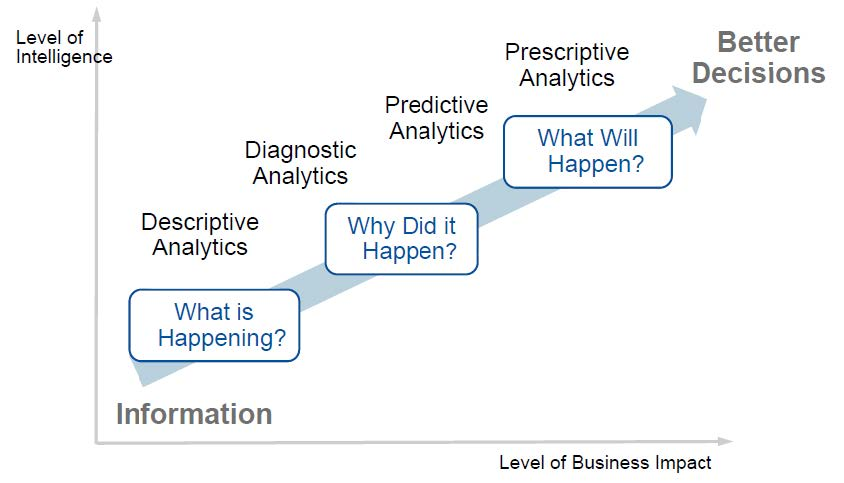
\includegraphics[width=\textwidth]{fig/analyseformen}
		\caption{Analyseformen von Big Data}
		\label{fig:analyseformen}
	\end{subfigure}
	~
	\begin{subfigure}[b]{0.4\textwidth}
		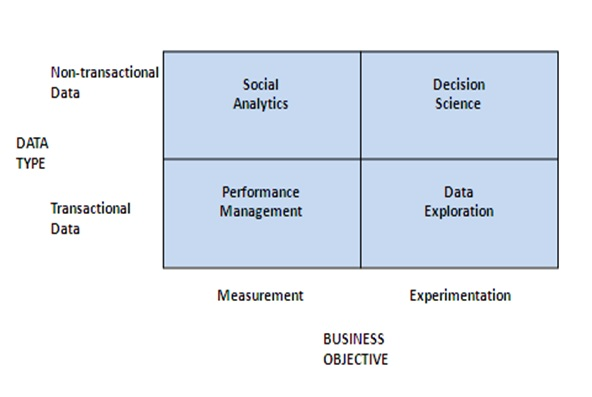
\includegraphics[width=\textwidth]{fig/strategy_bigdata}
		\caption{Strategien zum Einsatz von Big Data}
		\label{fig:strategy_bigdata}
	\end{subfigure}
\end{figure}


\end{document}